\documentclass[a4paper, oneside]{csthesis}

% package to be able to use special characters
\usepackage[latin1]{inputenc}

% Sophisticated math package
\usepackage{amsmath}

% Special symbols
\usepackage{amssymb}

% nicely render theorems and proofs
\usepackage[standard,thmmarks,amsmath]{ntheorem}

\usepackage{graphicx}

% package to format pseudo-code. Check the package documentation.
\usepackage{algorithmic}
\usepackage{algorithm}

% Provides \xspace command that evaluates to a space if the next character in the source is a blank and
% no space if next character is no blank. Useful in command definitions.
\usepackage{xspace}

% Provides a more flexible tabular environment
\usepackage{tabularx}

% Enables the use of the H location specifier for float environments that puts the float exactly where it is located in the source.
\usepackage{float}

% Enables the use of colours
\usepackage{color}

% Enable listings to embed code
\definecolor{lightgray}{gray}{0.95}
\definecolor{darkblue}{rgb}{0,0,.5}

\usepackage{listings}
\usepackage{courier}
\lstset{
         basicstyle=\footnotesize\ttfamily, % Standardschrift
         %numbers=left,               % Ort der Zeilennummern
         numberstyle=\tiny,          % Stil der Zeilennummern
         %stepnumber=2,               % Abstand zwischen den Zeilennummern
         numbersep=5pt,              % Abstand der Nummern zum Text
         tabsize=2,                  % Groesse von Tabs
         extendedchars=true,         %
         breaklines=true,            % Zeilen werden Umgebrochen
         keywordstyle=\color{red},
         frame=b,
 %        keywordstyle=[1]\textbf,    % Stil der Keywords
 %        keywordstyle=[2]\textbf,    %
 %        keywordstyle=[3]\textbf,    %
 %        keywordstyle=[4]\textbf,   \sqrt{\sqrt{}} %
         stringstyle=\color{white}\ttfamily, % Farbe der String
         showspaces=false,           % Leerzeichen anzeigen ?
         showtabs=false,             % Tabs anzeigen ?
         xleftmargin=17pt,
         framexleftmargin=17pt,
         framexrightmargin=5pt,
         framexbottommargin=4pt,
         backgroundcolor=\color{lightgray},
         showstringspaces=false      % Leerzeichen in Strings anzeigen ?
 }
\lstloadlanguages{% Check Dokumentation for further languages ...
         %[Visual]Basic
         %Pascal
         %C
         %C++
         %XML
         %HTML
         Ruby
 }
% \DeclareCaptionFont{blue}{\color{blue}}

  %\captionsetup[lstlisting]{singlelinecheck=false, labelfont={blue}, textfont={blue}}
\usepackage{caption}
\DeclareCaptionFont{white}{\color{white}}
\DeclareCaptionFormat{listing}{\colorbox[cmyk]{0.43, 0.35, 0.35,0.01}{\parbox{\textwidth}{\hspace{15pt}#1#2#3}}}
\captionsetup[lstlisting]{format=listing,labelfont=white,textfont=white, singlelinecheck=false, margin=0pt, font={bf,footnotesize}}

\captionsetup{format=listing,labelfont=white,textfont=white, singlelinecheck=false, margin=0pt, font={bf,footnotesize}}

\usepackage{subcaption}

% Enables clickable links in the PDF and additional PDF specific configuration options.
\usepackage[
            colorlinks=true,
            linkcolor=darkblue, urlcolor=darkblue, citecolor=darkblue,
						raiselinks=true,
            bookmarks=true,
            bookmarksopenlevel=1,
            bookmarksopen=true,
            bookmarksnumbered=true,
            hyperindex=true,
            plainpages=false,
            pdfpagelabels=true,
            pdfstartview=FitH,
            pdfstartpage=1,
            pdfpagelayout=OneColumn
            ]{hyperref}




% link to website in footnote automatically
\newcommand\fnurl[2]{%
  \href{#2}{#1}\footnote{\url{#2}}%
}

% Load own command definitions, a few helpful ones are already defined there.

% This alters the numbering of theorems and lemmas.
\theoremsymbol{\ensuremath{\scriptstyle \Diamond}}
\renewtheorem{theorem}{Theorem}[chapter]
\renewtheorem{lemma}[theorem]{Lemma}
\renewtheorem{corollary}[theorem]{Corollary}
\renewtheorem{definition}[theorem]{Definition}

% This creates a two new theorem-like environments
\theoremsymbol{}
\newtheorem{notation}[theorem]{Notation}
\theorembodyfont{}
\newtheorem*{problem}{Problem}

% This changes the comment style of the "algorithmic" pseudocode package
\renewcommand\algorithmiccomment[1]{\hfill \small \(\triangleright\) #1}

% This creates four commands to leave annotations in your document
\newcommand{\TODO}[1]{\noindent {{\color{red}\fbox{\sffamily \bfseries TODO}} \sffamily #1}}
\newcommand{\FIXME}[1]{\noindent {{\color{green}\fbox{\sffamily \bfseries FIXME}} \sffamily #1}}
\newcommand{\CONSIDER}[1]{\noindent {{\color{blue}\fbox{\sffamily \bfseries CONSIDER}} \sffamily #1}}
\newcommand{\RW}[1]{\noindent \color{blue}#1}


% enable dashed lines
\usepackage{etex}
\usepackage{arydshln}



%%%%%%%%%%%%%%%%%%%%%%%%%%%%%%%%%%%%%%%%%%%%%%%%%%%%%%%%%%%%%%%%%%%%%%%%%%%%%%%%%%%%%%%%%%%%%%%%%
% DOCUMENT METADATA

\thesistype{Master Thesis\\[5pt]CONFIDENTIAL}
\title{Fraud Prevention and Detection\\[5pt] in Mobile Payments}

\author{Cedric Waldburger}
\email{wcedric@ee.ethz.ch}
\institute{Distributed Computing Group \\[2pt]
Computer Engineering and Networks Laboratory \\[2pt]
ETH Zurich}

% You can put in your own logo here "\includegraphics{...}" or just comment the command
% \logo{}

\supervisors{Christian Decker\\[2pt] Conor Wogan (SumUp)\\[2pt] Prof.\ Dr.\ Roger Wattenhofer}

% You can comment the following two commands if you don't need them
\keywords{Fraud Detection, Signature Verification, Mobile Payments, Mobile Applications, Dynamic Time Warping, Hidden Markov Models}
% \categories{ACM categories go here.}

\date{\today}

%%%%%%%%%%%%%%%%%%%%%%%%%%%%%%%%%%%%%%%%%%%%%%%%%%%%%%%%%%%%%%%%%%%%%%%%%%%%%%%%%%%%%%%%%%%%%%%%%

\begin{document}

\frontmatter
\maketitle % do not remove this line

\cleardoublepage

\begin{acknowledgements}

  I would like to thank my advisors Prof. Roger Wattenhofer and Christian Deck from the Institute for distributed computing at ETH Zurich for their help and support. I also wish to thank Stefan Jeschonnek, Conor Wogan, Matti Biskup and the whole Software Development Team at SumUp for their continuous support and help.

\end{acknowledgements}


\begin{abstract}
    Mobile payments have seen a lot of traction recently and a wide variety of companies have emerged around the opportunity of payments processed from mobile devices. Our work was conducted in collaboration with a company that allows merchants to process credit card transactions on their smartphone by using a mobile application and hardware dongle.

    The innovative technology has opened up many new beneficial opportunities for both, merchants and clients. It has also opened new opportunities for fraud in the area of credit card transactions, an area which has always been prone to fraud. Although the industry is highly regulated, the advances in technology call for new anti-fraud measures.

    We identify two  separate but complementary methods against credit card fraud: \textbf{preventive}, in the form of an automatic, more in-depth check of all users during the sign-up process against a database of individuals with higher risk status, and \textbf{reactive} by providing mechanisms to check every transaction's signature in real time against the card holder's previous signatures.

    Our work has shown that the optimization of the check during sign-up is able to reduce the number of false positives by (TODO: XX percent). This results in up to (TODO: XX hours) less manual work by operations team each week.

    We found that the characteristics of a signature captured by finger on a mobile device are much less stable than those of signatures captured with a pen. Therefore, we propose to use a feedback loop to improve the reliability of the signature verification algorithm and reduce the EER of our algorithm which fuses the score of a DTW algorithm, an HMM and a score base on global features.

\end{abstract}

\tableofcontents

\mainmatter % do not remove this line


%%%%%%%%%%%%%%%%%%%%%%%%%%%%%%%%%%%%%%%% CHAPTER INTRODUCTION

\chapter{Introduction}

As smartphones become increasingly popular, they're being used in more and more industries and fields. An application that has seen a lot of traction recently is mobile payments. The usage of the smartphone in this field includes the utilization as an electronic wallet, a virtual bank account and as a payment processing terminal to accept credit cards and other payment methods.
This work focuses on an application of the latter.
% Although mobile payments were getting a lot of attention already 10 years ago \cite{5342298}, only recently as the density of smartphones has reached a critical level, the use of smartphones as electronic cash registers has become practical.
The density of smartphones per capita and the computational power of current mobile phones have reached a level where it became practical to use phones electronic cash registers.
\fnurl{iZettle}{http://www.izettle.com}, \fnurl{Square}{http://www.squareup.com}, \fnurl{SumUp}{http://www.sumup.com} are just some of the companies which make use of this situation and are enabling merchants to receive payments via their smartphone. This thesis was written in collaboration with SumUp, a mobile payment company located in Berlin.

% \cite{Hanmandlu05} \cite{citeulike:3393241} \cite{citeulike:885135} \cite{1030918} \cite{1227706} \cite{Kim:2005:SED:2156512.2156558} \cite{Coetzer:2004:OSV:1289340.1289385} \cite{711942}

Financial businesses have a higher risk of being the target of fraud attacks than businesses in other industries due to the direct financial gain for fraudsters. On mobile devices, it becomes even more important to protect the system from fraud --- especially as the mobile devices can be lost or stolen. While some security measures are imposed by financial authorities, those rules were made for traditional financial institutions. The new mobile, connected environment not only opens up a lot of beneficial opportunities but also more attack vectors for fraudsters. Therefore it is important to not only respect given guidelines but pro-actively look for ways to prevent possible attacks.

We focused our work on two separate, complementary approaches to reduce the fraud risk for a mobile payment company like SumUp.
Thanks to implementing an in-depth check of new users during the sign-up process, we preventively reduced the risk of signing up a high risk account. After screening a new user, suspicious applications are flagged for manual inspection of the information that caused the flagging. As this reduced the amount of accounts that have to be checked manually, we were able to reduce the amount of manual work per sign-up substantially.
Going forward, we refer to the preventive part of our work as "fraud prevention" and the reactive part as "fraud detection". We use the term "fraud protection" for findings that apply to both, fraud prevention and detection.

Our second approach focused on reactive fraud detection and makes use of the most popular method to authorize credit card transactions in mobile payments: by signature.
Authorization of credit card transactions can be done in various ways. They differ in terms of technical complexity and thus cost, speed at which a transaction can be processed and acceptance by card schemes. The most popular card schemes in Europe are MasterCard, VISA, American Express, Diner's Club and others. Widely used are the three following methods:

\begin{itemize}
\item Swipe And Signature (SAS): The card holder swipes his card through a card reader and the transaction is confirmed by signature on the mobile device. Low technical complexity but easy to attack as the data on the magnetic stripe is not encrypted. Main problem: cards can be copied while the card data is read. Widely deployed in the USA due to high acceptance by Card Schemes.
\item Chip And Signature (CAS): The card holder inserts his card into a card reader and the encrypted data is read from the card's chip. The user authorizes the transaction by signature on the smartphone screen. This is currently the most popular method to authorize payments in Europe on mobile devices. CAS' biggest drawback is that Visa Europe, even though the technical complexity for such readers is much higher, does not consider this method secure enough and therefore requires an extended flow that requires the client to confirm the transaction with a text message. Except from Visa Europe, all other card schemes consider CAS to be secure enough.
\item Chip And Pin (CAP): A card holder inserts the card into a card reader and enters his Personal Identification Number (PIN) into the reader's pin pad to authorize the transaction. Only after the correct PIN has been entered, the phone is able to read the necessary data to process the transaction. The main drawback of this authorization method is its high technical complexity in the reader and on the server side and thus high costs incurred by the hardware and software. Although this process would allow to process any card schemes in Europe, the high cost make a widespread use in the short term unlikely.
\end{itemize}

Although authorization with CAS is a lengthy process with VISA cards in Europe, it is currently the best compromise between speed, cost and an almost universal acceptance by card schemes. SumUp provides merchants with SAS readers or CAS readers based on the merchant's profile. This means that currently, all signatures are authorized by signature. Also with other providers of the same service, authorization by signature remains the predominant way to authorize transactions.

We propose an automatic signature verification system based on a set of global features, Dynamic Time Warping (DTW) and Hidden Markov Models (HMM) to make the authorization process more secure. As the signatures, which are captured by finger, tend to have a high variability and unstable characteristics, our system has to account for false positive matches. To account for that, we propose a system involving a feedback loop. With a feedback loop, transactions are still possible even if a card holder's signature could not be matched to previous signatures.





\section{SumUp - Mobile Payments for Everyone}
\label{intro-sumup}

Credit cards enjoy a huge popularity among consumers which is illustrated by the number of credit card holders in the United States of America (USA) only: In 2008 over 176.8 million people owned a credit card with average of 3.5 cards per card holder. About 60 percent of consumers own a rewards credit card and approximately 51 percent of the USA's population owns at least two credit cards.\cite{woolsey2010credit}

While credit cards are also very popular with consumers in Europe, far fewer businesses in Europe allow customers to pay by credit card than in the USA. This is mostly due to the following reasons:
\begin{itemize}
\item A European business initially pays between 200 EUR to 500 EUR for a credit card terminal
\item There is a monthly subscription fee from 20 EUR to 50 EUR
\item A percentage of each transaction goes to the credit card company. Usually, merchants pay between 2.75 and 5 percent to the card payment terminal provider.
\end{itemize}

It is likely that these costs are higher due to more complex regulations and more complex payment terminals required by the card schemes in Europe.

SumUp's goal is to lower the barrier for merchants to accept credit card payments by providing a professional yet inexpensive solution for anyone to accept card payments. The company was founded in the fall of 2011 and has enjoyed a rapid growth since.
Today, SumUp's services are used by thousands of merchants in more than ten European countries.
The business has been successful because it removed two out of three of the previously mentioned obstacles to a more widespread adoption: anyone who signs up with SumUp receives a free card reader for use with a smartphone and there is no monthly subscription fee. As the merchant already owns the expensive hardware in form of a smartphone and most people already pay for a data subscription, the cost on both ends is much lower. This way, SumUp is able to finance itself through the 2.75 percent transaction fee. At its core, it competes with traditional Credit Card Terminal companies who require their users to pay a monthly fee for their terminal and the expensive initial charge for the device.

Instead of building and selling expensive hardware, the only hardware required --- the card reader --- is shipped at no charge and the software is distributed for free via the Apple AppStore and Google Play Store.
Payment through SumUp gives taxi drivers, market traders and other small stores, who couldn't afford one of the traditional payment terminals, an enormous economic advantage, in that mobile payments can now be processed right on the spot and without an initial financial investment.


Processing a transaction with SumUp is illustrated in five simple steps in Fig \ref{fig:flow-customer}.

\begin{figure}
        \centering
        \begin{subfigure}[b]{0.16\textwidth}
                \centering
                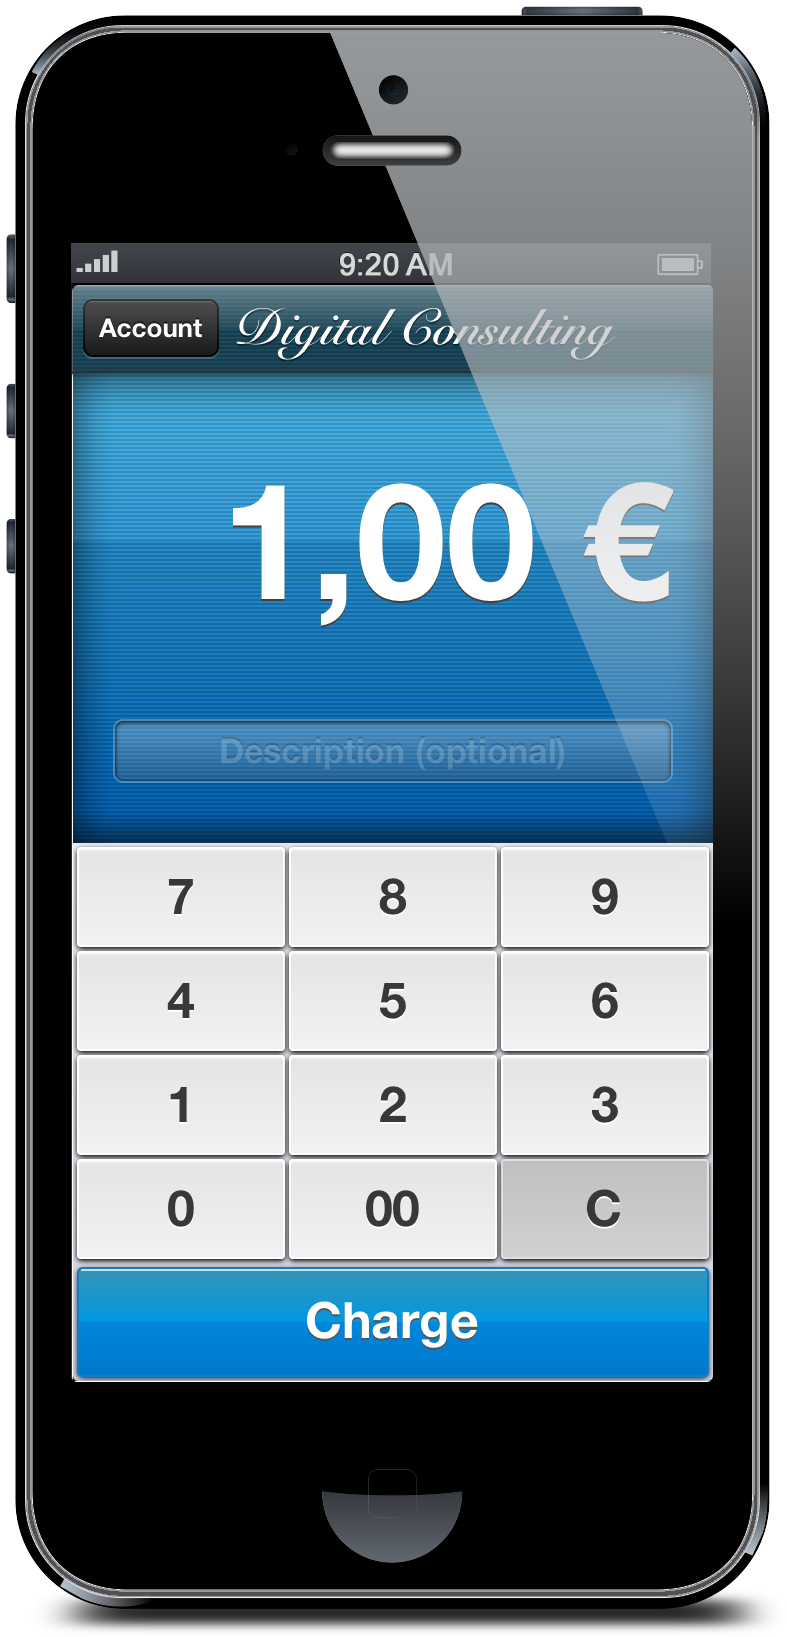
\includegraphics[width=\textwidth]{figures/flow1.png}
                % \caption{Merchant enters amount nto digital cash register}
                \label{fig:flow1}
        \end{subfigure}%
        ~ %add desired spacing between images, e. g. ~, \quad, \qquad etc.
          %(or a blank line to force the subfigure onto a new line)
        \begin{subfigure}[b]{0.16\textwidth}
                \centering
                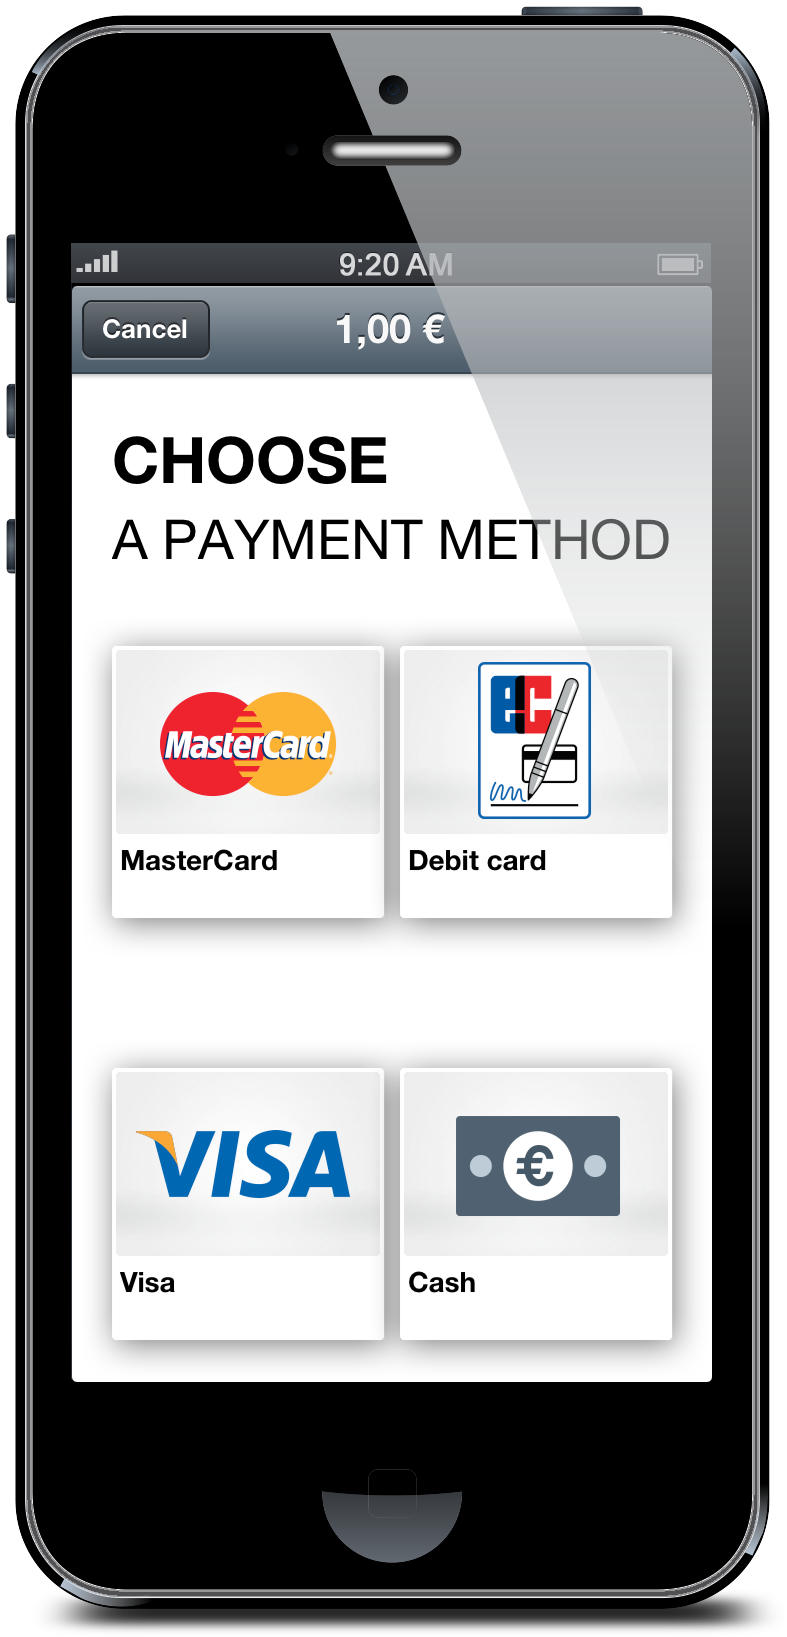
\includegraphics[width=\textwidth]{figures/flow2.png}
                % \caption{Merchant chooes the payment method}
                \label{fig:flow2}
        \end{subfigure}
        \begin{subfigure}[b]{0.16\textwidth}
                \centering
                
\includegraphics[width=\textwidth]{figures/flow3.png}
                % \caption{Once the card reader has been plugged in, the device is ready to read a card}
                \label{fig:flow3}
        \end{subfigure}
        % \begin{subfigure}[b]{0.12\textwidth}
        %         \centering
        %         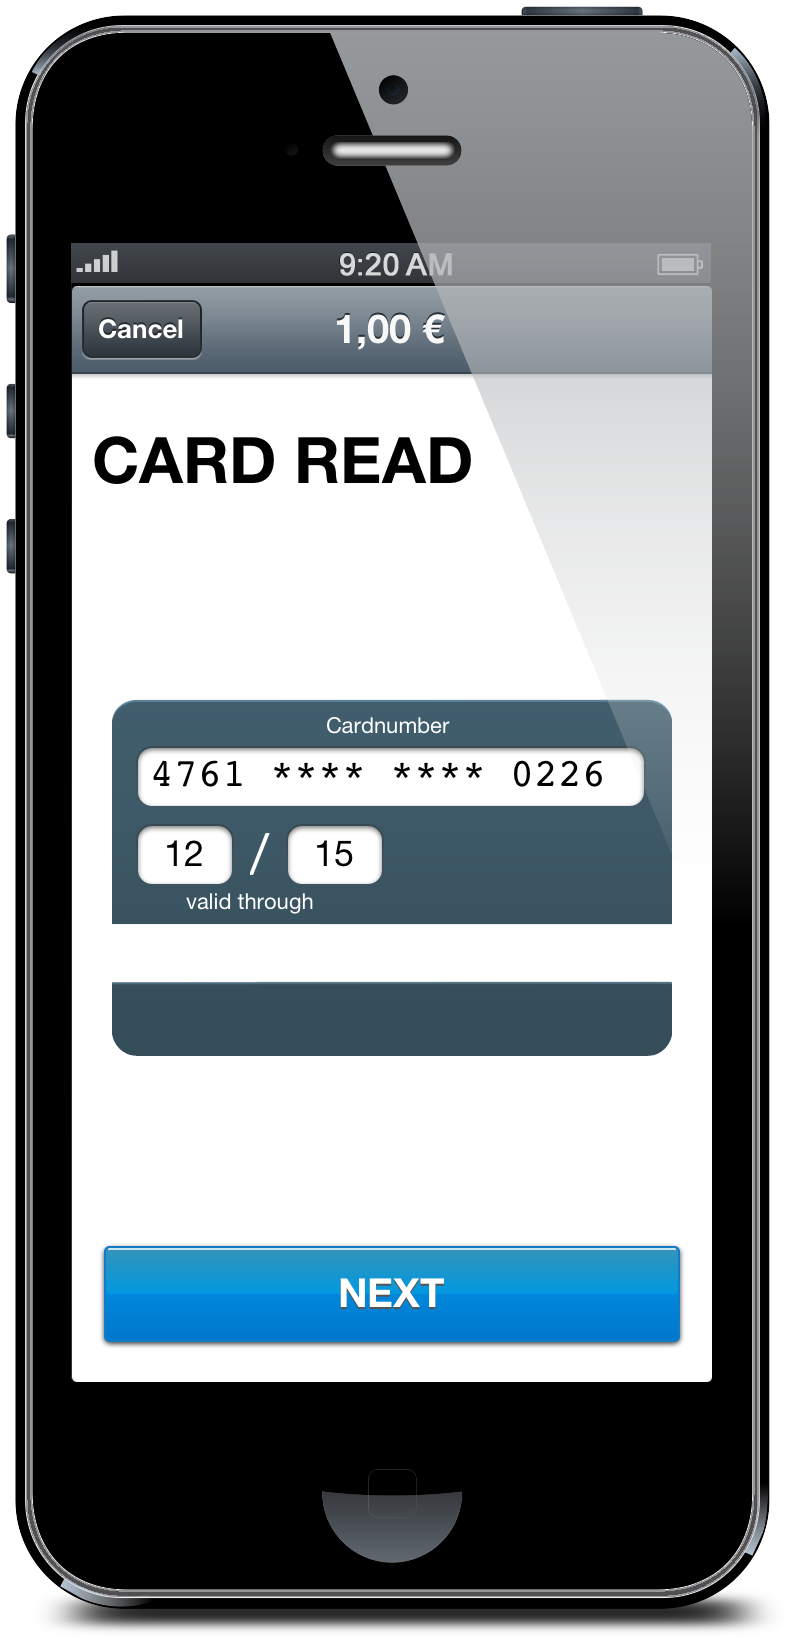
\includegraphics[width=\textwidth]{figures/flow4.png}
        %         % \caption{Card is recognized and shown on the screen}
        %         \label{fig:flow4}
        % \end{subfigure}
        \begin{subfigure}[b]{0.3\textwidth}
                \centering
                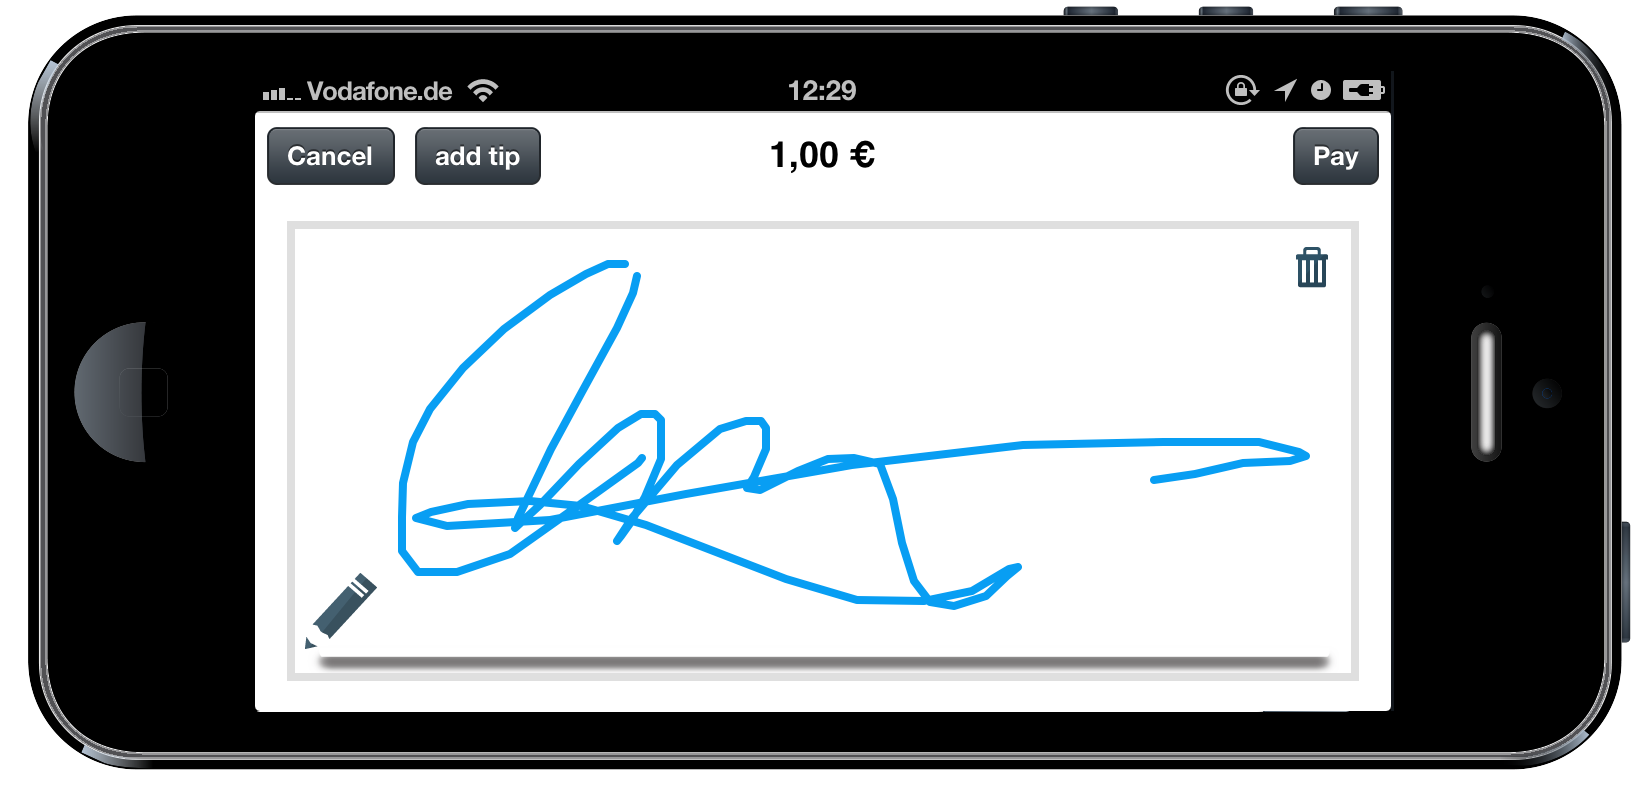
\includegraphics[width=\textwidth]{figures/flow5.png}
                % \caption{Customer signs and thereby confirms transaction}
                \label{fig:flow5}
        \end{subfigure}
        \begin{subfigure}[b]{0.16\textwidth}
                \centering
                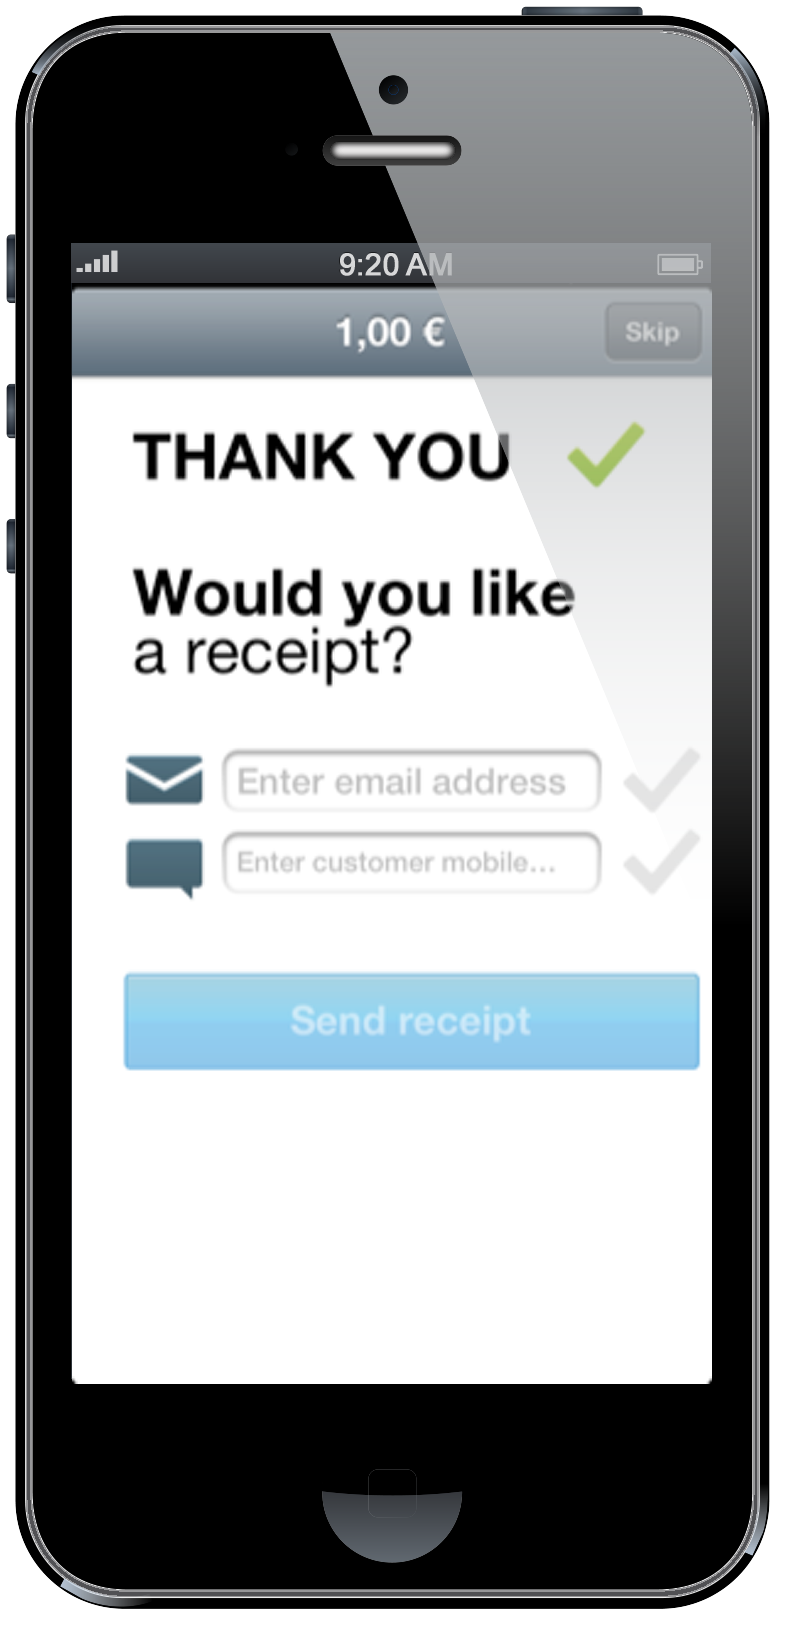
\includegraphics[width=\textwidth]{figures/flow6.png}
                % \caption{Customer can choose to receive a receipt via email or text}
                \label{fig:flow6}
        \end{subfigure}
        \caption{In-App Flow during a Transaction from step 1 to step 5 (from left to right)}\label{fig:flow-customer}
\end{figure}

\begin{enumerate}
\setcounter{enumi}{-1}
    \item Once the merchant has registered a SumUp Account and provided identification documents, he receives a free card reader and can accept payments.
    \item The purchase amount can be entered manually into the mobile application or via previously created products
    \item Debit cards and credit cards like Visa and MasterCard are supported and can be chosen by clicking on the respective logo.
    \item After reading the card, the mobile application shows a confirmation of the card type and number.
    \item The customer confirms the transaction with a signature written onto the screen of the smartphone or tablet.
    \item After successful completion, the customer can have the receipt sent to their email account or via SMS to their phone.
\end{enumerate}


Depending on the authorization method, a number of requests are made towards the SumUp servers and from there to other components of the transaction authorization chain, including acquirers, issuing banks and credit card institutions. Internally, a request is sent to SumUp's fraud server which performs a variety of checks and analysis to decide whether or not the transaction is accepted or declined. There's currently no established third party provider for fraud detection in this area and all rules are custom made by each company. The signature is part of the data that is exchanged with the fraud server and the signature verification process as described in Chapter \ref{chp:signature-verification} is an integral part of the  authorization process.

Along with simplicity, quick setup time and low cost, SumUp's advantage over its competitors is that it deducts a relatively low fee per transaction of 2.75\%. From that fee, it also pays the other parties in the value chain. To build a sustainable business model, SumUp will enable customers to also process other types of mobile payments, alongside credit card transactions. The Consumer-To-Business credit card transactions will only be one part of all mobile payment transactions. A long term strategy is to implement all payment schemes as listed by the European Payments Council (EPC). Mobile payments may at one point replace all current payment methods for Business-to-Consumer (B2C) transactions as well as Business-to-Business (B2B), Consumer-to-Business (C2B) and Consumer-to-Consumer (C2C) transactions as listed with examples in Table \ref{fig:mp-applications}. The EPC predicts this will happen due to the availability and convenience of mobile devices paired with the user's perception of having full control over it. This creates an environment of trust and convenience for conducting payments. \cite{mpwhitepaper}


\begin{figure}
        \centering
        \begin{tabular}{c|l}
        \hline
% & 0 & 0 \\ \hline
C2C & Repay a friend \\ \hdashline[0.5pt/3pt]
C2B & Buy Groceries \\ \hdashline[0.5pt/3pt]
B2C & Pay for train to work with company account \\ \hdashline[0.5pt/3pt]
B2B & Pay for Business Lunch \\ \hline
        \end{tabular}
        \caption{Examples of mobile payment applications as listed by the EPC}\label{fig:mp-applications}
\end{figure}


% So funktioniert SumUp:
% Identifizieren und Kartenleser bekommen: Lassen Sie sich mit dem angehängten Formular per Postident identifizieren und wir schicken Ihnen den kostenlosen SumUp Kartenleser zu.
% Starten: Jetzt können Sie Zahlungen von EC- und Kreditkarte empfangen. Nachdem bereits 40% aller Zahlungen mit Karte getätigt werden, verpassen auch Sie nun kein Geschäft mehr! Ob im heimischen Betrieb oder mobil, kein Spontankauf wird mangels Bargeld ausfallen.
% Geld empfangen: Auszahlungen auf Ihr Konto erfolgen jeden Tag, sobald Sie eine Schwelle von nur 20€ Umsatz erreicht haben.
% Kosten: SumUp berechnet eine Gebühr von 2,75% pro Kartenzahlung. Ohne Vertragslaufzeit, ohne Mindestgebühr, ohne Einrichtungsgebühr, ohne monatliche Kosten.


\section{Fraud}

Fraud, as defined by Phua et al. ~\cite{5522816}, refers to the abuse of a profit organization's system without necessarily leading to direct legal consequences. Fraud detection, as part of the overall fraud control, has become one of the most established applications of data mining.

The large volume of transactions processed each day by SumUp make a manual verification of each transaction impossible. As such, SumUp has to rely on automated systems to process and validate transactions. At time of this research, there is no established provider of anti-fraud software in this field. However, companies like \fnurl{Sift Science}{http://siftscience.com}, a company that specializes in providing a fraud control service as a third party, has recently raised more than four millions USD from leading venture capital firms.

At the time of this work, SumUp has internal research to implement, train and tweak its own fraud rules. An internal assessment has shown that the four most popular fraud scenarios are the following:

% As credit cards are historically a very unsafe payment method, special attention has to be paid when dealing with credit card information and processing credit card transactions.
% A fact that is reflected by looking at how many papers were written about fraud detection in which area. As shown in Figure \ref{fig:fraud-literature-count}.

\begin{itemize}
    \item Copied or stolen cards
    \item Money laundry
    \item Impersonators transferring money under someone else's name
    \item Illegal money being transferred through SumUp's system
\end{itemize}

We will mainly focus on the first fraud case and concentrate on identifying a card holder by signature. After a card has been used a certain amount of times, the goal is to  build a reliable signature model to verify it's the same person signing the next time the card is used.

Not only the physical cards are at risk to be stolen, also the digital copy of the credit card data needs to be protected. This is one of the reasons SumUp only saves encrypted card information and is obliged to do so according to the Payment Card Industry Data Security Standard (PCI DSS) and in an environment defined by the standard. The standard defines a set of rules to reach these control objectives:
\begin{itemize}
\item Build and maintain a secure network
\item Protect card holder data
\item Maintain a vulnerability management program
\item Implement strong access control measures
\item Regularily monitor and test networks
\item Maintain an information security policy
\end{itemize}

This has an impact on our work as the regulations connected to  protecting card holder data only allows storing card numbers and not names of card holders. The goal of this requirement is that even if someone would gain access to SumUp's database, it would not be possible to retrieve all information needed to process a transaction. This has one disadvantage though: we cannot collude information of multiple cards used by a single customer and can therefore only build a signature model based on the signatures we collect per card, not per customer. As the majority of all US card holders holds at least two credit cards \cite{woolsey2010credit}, being able to merge the signature databases from different cards of one card holder, could significantly increase the accurateness of the signature model.

It is impossible to be absolutely certain about the legitimacy of a transaction. In reality, the goal must be to filter out possible evidences of fraud from the available data using cost-effective algorithms in real time.



% \begin{figure}[tb]
%     \begin{center}
%         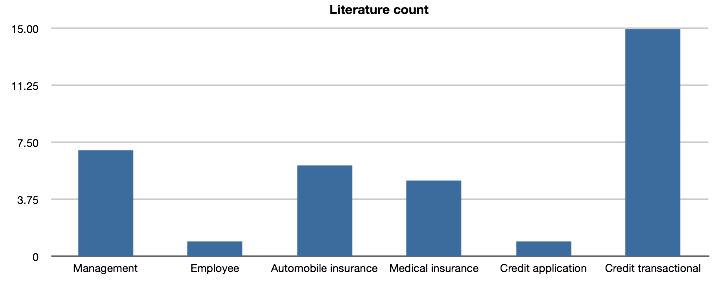
\includegraphics[width=\textwidth]{figures/fraud-literature-count}
%     \end{center}
%     \caption{Number of research papers published on different fraud areas}
%     \label{fig:fraud-literature-count}
% \end{figure}





\section{Signature Verification}

Most previous work has been done on signature verification with signatures captured with a pen on paper or on a digital tablet. When a signature was captured on paper, it was afterwards digitalized using a scanner. The dynamic characteristics of a signature are lost in that process and the algorithms that can be applied to the signature information are very different. Therefore it is common to divide signature verification methods into two methods:

\begin{itemize}
\item \textbf{Offline signature verification} performs recognition algorithms based on static features of a signature, mainly shape and length.
\item \textbf{Online signature verification} performs algorithms on the dynamic features of a signature as well. These analyze the speed, the acceleration, the angular acceleration, the pressure and many other local properties of a signature.
\end{itemize}

Since digital tablets, touchscreens interfaces and smartphones became affordable and widely deployed, it became feasible to capture dynamic features of a signature. In Chapter \ref{chp:signature-verification} we look at the common techniques in both areas, offline and online, to verify signatures.

The high accuracy and resolution of current digitizing tablets and smartphone screens enables to capture signature data in high resolution and precision on relatively cheap devices.
Traditionally, digital signatures were captured on a digital tablet with a pen. Signatures captured by SumUp however, are collected on a variety of mobile devices and have fundamentally different characteristics than signatures captured on a digital tables. The main reasons for these differences are:

\begin{itemize}
    \item The signatures are captured by finger instead of a pen which is not how people are accustomed to sign. This leads to higher variability and less stable signature models.
    \item Most smartphones don't have a fixed sampling rate but an event-based sampling. Whereas the sampling rate on digital tablets is constant, the rate in signatures captured on smartphones can vary a lot within one signature.
    \item The signatures are captured on a lot of different devices with different screen sizes, resolutions, sensor densities and other device specific characteristics.
\end{itemize}

We have to verify signatures within a fraction of a second to give instant feedback whether or not a transaction will be authorized. This limits not only the number of algorithms we can use in parallel but also the complexity of our models and our dataset.
We discuss our strategies to overcome the listed difficulties in Chapter \ref{chp:signature-verification}.

% How to approach that without the complicated and expensive chip\&pin device?

% Use signature detection to determine if someone is who he/she claims to be

% Specialties of Mobile Payment Signatures:
% - They don't need to be extracted from a paper background
% - All the info is available (timestamps), digital

% Diverse applications inspired researchers to investigate the feasibility of two distinct categories of automatic signa- ture verification systems: those concerned with the verifica- tion of signature images and those concerned with the veri- fication of signatures that were captured dynamically, using a special pen and digitising tablet. These systems are referred to as offline and online systems, respectively.

% In offline systems, a signature is digitised using a hand- held or flatbed scanner and only the completed writing is stored as an image. These images are referred to as static sig- natures. Offline systems are of interest in scenarios where only hard copies of signatures are available, for example where a large number of documents need to be authenti- cated.
% In the online case, a special pen is used on an electronic surface such as a digitiser combined with a liquid crystal dis- play. Apart from the two-dimensional coordinates of succes- sive points of the writing, pen pressure as well as the angle and direction of the pen are captured dynamically and then stored as a function of time. The stored data is referred to as a dynamic signature and also contains information on pen velocity and acceleration. Online systems are of interest for “point-of-sale” and security applications.

% Since online signatures also contain dynamic informa- tion, they are difficult to forge. It therefore comes as no sur- prise that offline signature verification systems are much less reliable than online systems.


% Various pattern recognition techniques have been ex- ploited to authenticate handwritten signatures (see Section 2). These techniques include template matching techniques [7, 9, 11], minimum distance classifiers [10, 12, 14, 15], neu- ral networks [8, 13, 16], hidden Markov models (HMMs) [17, 18], and structural pattern recognition techniques.
% => p559 coetzer

% Jose L Camino:
% Usually the signature classification methods are divided into two kinds: On-line systems and off- lines systems. The on-line systems parameterize the signature using dynamic characteristics such as how long is the signing process, the inclination of the pencil when signing, the pressure on the pencil on the sheet, the speed of the written line, etc. For that, an electronic pencil is used [4][5][6]. Subsequently a classifier is used to recognize the signature form above parameters. In off-line classification method the signature is written on a sheet and it is scanned. Subsequently, fiom the image scanned, the usual step is parameterize their geometric structure as previous stage to their recognition by a Neural Network based classifier [2,7,8,9].



%%%%%%%%%%%%%%%%%%%%%%%%%%%%%%%%%%%%%%%% CHAPTER FRAUD


\chapter{Fraud Prevention \\PEP \& HRA Detection}

The fraud prevention is applied during the sign-up process of a new user and with the goal to keep high risk users from gaining access to the system.
Any financial institution has a high interest to implement as many anti-fraud mechanisms as possible. With the financial industry being a strictly regulated industry, many precautions are mandatory and described by the governing financial authority. Yet, more mechanisms are added on top of the mandated ones as they provide a competitive advantage.

The financial authority governing SumUp's operations is the United Kingdom (UK) Financial Services Authority (FSA) and the regulatory environment is specified in the Money Laundry Regulations (MLR) from 2007 ~\cite{website:aml-regulations-2007}. Chapter 2 of the MLR specifies the due diligence that has to be done for every client. As part of the due diligence process, the financial institutions are required to check that the customer does not fall into one of the two following categories:

\begin{itemize}
\item \textbf{Politically Exposed Persons} (PEP) are people who hold a prominent political function. In the United Kingdom this is defined as a national position. Also a PEP's spouse and children are included in this category.

\item \textbf{High Risk Accounts} (HRA) are people who have previously committed a financial crime, been involved in a money-laundering related crime (e.g. dealing with narcotics) or are listed on a government watch list.

\end{itemize}

We will refer to the combination of PEP and HRA as "high risk clients". Any new client needs to be checked against both lists at sign-up and regularily after the initial sign-up.
If the algorithm returns a positive match with either a PEP or an HRA, a flag is raised in the SumUp Operations Admin Panel (SOAP) and the match has to be confirmed or falsified manually. If the match can be falsified, nothing more needs to be done and the user will continue the sign-up flow. However, if there is a positive PEP or HRA match, different procedures have to be followed.

For an identified PEP match, additional due diligence needs to be done to onboard the client. Additional documents need to be collected that give detail information about the wealth and assets of said person. After performing the additional due diligence, a client can be onboarded but settlements need to be blocked.
A positive match with the HRA list means that the subject cannot be onboarded and a Suspicious Act Report (SAR) needs to be filed with the Serious Organized Crime Agency (SOCA). All HRAs are banned from conducting business with any financial institution.

Previous to our work, a test based on only first and last name was already in place but produced a lot of false positives. This required a lot of manual work to falsify matches. Our goal was to create a fast, reliable check requiring as little manual input as possible. Chapter \ref{chp:experiments} lists our results.

In the next section we'll present the data of the two databases and their origin before talking about the way we structured the lookup and implementation of our solution.

% two strat agains aml: identify customer, get id \& proof of address
% 2nd mitigating strategy: monitor patterns, activity, ...

% plugged into both: screening at beginning \& end


% sanctions hit => can't trade with him
% report suspicion report

% suspicious act report = sar

% => serious organized crime association

% pep = enhanced customer due diligence
% get more docs, based on wealth and funds

% if we onboard them, we need to block settlements


% Our work is inspired by, amongst others, the potential fi- nancial benefits that the automatic clearing of cheques will have for the banking industry. Despite an increasing num- ber of electronic alternatives to paper cheques, fraud perpe- trated at financial institutions in the United States has be- come a national epidemic. The National Check Fraud Center Report of 2000 [1] states that: “. . . cheque fraud and coun- terfeiting are among the fastest-growing crimes affecting the United States’ financial system, producing estimated annual losses exceeding USD 10 billion with the number continuing to rise at an alarming rate each year.”

% 1: National Check Fraud Center, National Check Fraud Center Report, 2000.

\section{PEP \& HRA Database}


World-Check \cite{website:world-check} is one of the providers of the PEP \& HRA database. It consolidates the list by polling many different lists - including the FBI's Most Wanted LIist, Interpol and others.

The data is supplied in a text file as Comma Separated Values (CSV) and contains information in 26 fields per person. The most important fields are listed in table \ref{tbl:world-check-fields}. Unfortunately, the records are far from complete. A lot of the records are missing some of the important fields like birthday or locations, which makes it hard to falsify a match automatically and sometimes a match falls back on just first and last name correlation. World-Check normalizes the data so that all dates have the same format, city and country names are always spelled the same name and data in one field is always represented the same way.

\begin{table}
    \begin{tabular}{l|p{9cm}}
    \hline
    Field & Value \\ \hline
    uid & unique identifier within the World-Check database\\ \hdashline[0.5pt/3pt]
    last\_name & subject's primarily used last name\\ \hdashline[0.5pt/3pt]
    first\_name & subject's primarily used firs first name \\ \hdashline[0.5pt/3pt]
    aliases & other first/last name combinations that the subject has used\\ \hdashline[0.5pt/3pt]
    alternative\_spelling & alternative spelling of the subject's name\\ \hdashline[0.5pt/3pt]
    category & used to define if subject is a PEP or HRA\\ \hdashline[0.5pt/3pt]
    sub\_category & used to define if subject is a PEP or HRA\\ \hdashline[0.5pt/3pt]
    age & age of the subject \\ \hdashline[0.5pt/3pt]
    dob & the subject's date of birth \\ \hdashline[0.5pt/3pt]
    deceased & information about the subject's death \\ \hdashline[0.5pt/3pt]
    locations & the cities the subject was associated with \\ \hdashline[0.5pt/3pt]
    countries & the countries the subject was associated with \\ \hdashline[0.5pt/3pt]
    further\_information & description and references about the subject \\ \hdashline[0.5pt/3pt]
    external\_sources & information about from which sources the information in the database was extracted \\ \hline

    \end{tabular}

    \caption{Fields of the World-Check database CSV file}
    \label{tbl:world-check-fields}
\end{table}


The full database file is about three gigabytes in size and contains some 1.8 million records of PEPs and HRAs combined. As the database is constantly changing, there's also a daily, weekly and monthly incremental update and delete file, with which the database is kept updated without having to download the full database file every so often.
World-Check is a paid service and the data is retrieved over encrypted HTTPS connection.




\section{Algorithm}

Clearly, parsing three gigabytes of raw data and rebuilding the database each time a new user processes through the sign-up flow is slow and not practical. We therefore chose to parse the needed data into a relational database, allowing us to perform queries within split seconds. The algorithm we used to make the lookup faster, consists of two parts - parsing and lookup.

\textbf{Parsing the data}

The raw data contains only one record per individual but often lists not only one pair of first and last name but many. The additional pairs are retrieved from the aliases and alternative\_spellings fields. For faster lookup, each record from the original CSV file is parsed into multiple records in the database such that there exists one database record for each pair of first and last name combination. We create a record for each permutation of first and last name retrieved from those fields to cover all identities a high risk user might possibly use.
Listing \ref{lst:world-check-parse} shows the algorithm used to create the cross product of all name pairs.

\textbf{Lookup}

To improve the duration of a lookup, the database has an index on first and last name on the PEP/HRA table to speed up the lookup. An index was also generated on the other fields used by the lookup algorithm: Date Of Birth (DOB), deceased, locations (cities) and countries.

To reduce the number of false positives, the lookup uses additional information besides the first and last name to confirm or falsify a match. For each lookup, at least the following information needs to be provided to the algorithm:
\begin{itemize}
\item First and last name
\item Date of birth
\item City
\item Country
\end{itemize}

The algorithm is outlined in Listing \ref{lst:world-check-lookup}. It's output is a set of Know Your Customer (KYC) action and statuses which flag the customer in the system and may restrict him from certain actions, e.g. processing transactions with her account.

\begin{lstlisting}[caption={The Lookup algorithm},label={lst:world-check-lookup}]
def lookup fname, lname, dob, city, country

    # collect all hits on first and last name
    all_hits = verified_hits = []
    all_hits << PEP.find_by_first_name_and_last_name(fname, lname)
    all_hits << HRA.find_by_first_name_and_last_name(fname, lname)

    for record in all_hits

        # skip if peson is already deceased
        next if record["deceased"]

        # parse dob. if the dob in the db is incomplete (eg 1971/02/00)
        # only check the complete parts
        y = record["dob"].year  != 0 ? record["dob"]["year"]  : null
        m = record["dob"].month != 0 ? record["dob"]["month"] : null
        d = record["dob"].day   != 0 ? record["dob"]["day"]   : null

        # now skip if one of the values exists but doesn't match
        next if y && y != dob["year"]
        next if m && m != dob["month"]
        next if d && d != dob["day"]

        # at this point, dob matches or wasn't given
        # now, check city
        next unless record["locations"].contains? city

        # and country
        next unless record["countries"].contains? country

        # all checks passed, add this record to the result set

        verified_hits << record

    end

    # now set KYC status for the proven records
    for r in verified_hits
        set_kyc_status r
    end
end
\end{lstlisting}


\section{Implementation \& Architecture}

The PEP \& HAR check was implemented as a \fnurl{Sinatra}{http://www.sinatrarb.com/} Ruby Applicaton, accessible through a REST interface. It fulfills multiple purposes: It parses the initial or incremental database file, it continuously rechecks all users in the database versus the updated database and also answers requests from the sign-up component.

It uses Ruby \fnurl{ActiveRecord (AR)}{http://guides.rubyonrails.org/active_record_querying.html} to connect to a relational database. The Ruby Sinatra Application runs within a \fnurl{CentOS}{http://www.centos.org/} Linux environment and the linux \fnurl{Crontab Tool}{http://unixhelp.ed.ac.uk/CGI/man-cgi?crontab+5/} is used to run the first two tasks in a constant interval:
\begin{itemize}
\item \textbf{daily:} Each day, the incremental update and delete file are downloaded from World-Check to keep the database up to date.
\item \textbf{weekly:} On a weekly base, each user is screened against the updated database and new hits raise a flag in SOAP.
\end{itemize}

The third task, answering requests from the sign-up flow is done via a REST interface. Chapter \ref{chp:experiments} goes into greater detail of how the requests are structured. The system topology is shown in Figure \ref{fig:fraud-arch}.

\begin{figure}[tb]
    \begin{center}
        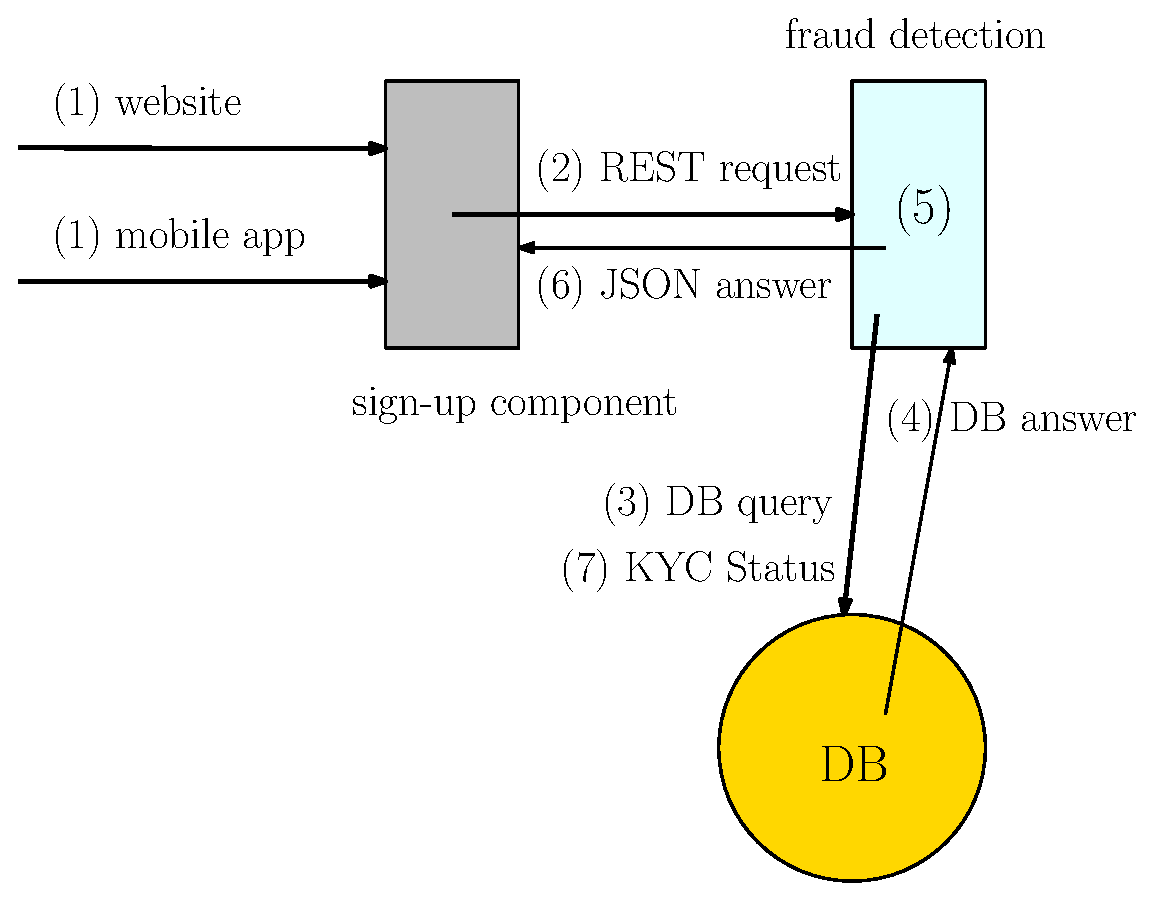
\includegraphics[width=0.8\textwidth]{figures/fraud-arch.eps}
    \end{center}
    \caption{The simplified architecture and strucutre of a PEP/HRA check request}
    \label{fig:fraud-arch}
\end{figure}

A request is triggered and answered with the following steps:

\begin{enumerate}
\item A new user signs up from one of the mobile apps or the website
\item The sign-up component sends a request for the new user to the fraud detection component
\item The component retrieves the necessary data from the database
\item The database delivers all matches based on first and last name
\item The Lookup algorithm is performed within the fraud detection component
\item The result is returned to the sign-up component with information of whether or not the user can continue the sign-up flow
\item The respective KYC actions and statuses are set in the database.
\end{enumerate}

TODO: Add performance improvement/performance data in Experiments chapter












%%%%%%%%%%%%%%%%%%%%%%%%%%%%%%%%%%%%%%%% CHAPTER Signature Recognition

\chapter{Fraud Verification \\Signature Verification}
\label{chp:signature-verification}

For centuries, being able to authenticate someone based on biometrics, has been important to conduct business, identify each other and connect written information with an author. In order to guarantee someone's identity, it has always been important to work towards more exact, more reliable means to measure someone's biometric properties. The characteristic properties of a handwritten signature help to prove a signer's identity. A signature has four legal properties: \cite{Hanmandlu05}

\begin{itemize}
\item \textbf{Authentication}: Signature verification allows to confirm a signer's identification
\item \textbf{Acceptance}: By signing a document, the writer conveys a willful intent and acceptance of the document's terms and contents
\item \textbf{Integrity}: By signing a document, the signer establishes the integrity of the signed document and that it has not been altered
\item \textbf{Non-repudiation}: The above three factors make it impossible for the signer to deny having signed the document
\end{itemize}

Signature verifications is a particularly important biometric identification process as the signature is a widely accepted method for endorsing financial transactions ~\cite{1227706}.
As the signature is recorded in the SAS and CAS authorization process, it makes sense for SumUp to use this information to improve the security of both authorization methods.

We present existing methods and related work before describing the signature verification methods used in our work and the peculiarities for signature detection in mobile payments.
Traditionally, detection methods can be assigned to either feature- and function-based methods. We describe both approaches in Section \ref{sec:features} and Section \ref{sec:functions}. As a combination of feature- and function-based approaches has been providing better results than the individual techniques \cite{fierrez2005line}, we combine both approaches in our method to verify signatures.

% Theoretically, the problem of handwritten signature verification is a pattern recognition task used to discriminate two classes of original and forgery signatures. A signature verification system must be able to detect forgeries and to reduce rejection of genuine signatures simultaneously.

% Human signature verification (HSV) systems are usually built either on-line or off-line approaches, depending on the kind of data and application involved. On-line systems generally present a better performance than the off-line ones but require the necessary presence of the author during both the acquisition of the reference data and the verification process limiting its use of certain kind of applications.

% A great deal of work has been done in the area of offline sig- nature verification over the past two decades. A recent paper by Guo et al. [11] includes an extensive overview of previous work. Numerous methods and approaches are summarised in a number of survey articles. The state of the art from 1993 to 2000 is discussed in a paper by Plamondon and Srihari [5]. The period from 1989 to 1993 is covered by Leclerc and Pla- mondon [19] and the period before 1989 by Plamondon and Lorette [20]. Another survey was published by Sabourin et al. in 1992 [21]. A review of online signature verification by Gupta and McCabe in 1998 also includes a summary of some earlier work on the offline case [22].
% Earlier work on offline signature verification deals pri- marily with casual and random forgeries. Many researchers therefore found it sufficient to consider only the global fea- tures of a signature.



\section{Global Systems}
\label{sec:features}

Global systems, also called feature-based systems, are characterized by the fact that the feature vector consists of measurements that are based on the whole signature. Example features are listed in table \ref{fig:global-features}. Velocity, acceleration and position are usually looked at either combined or per dimension (usually $x/y$).



\begin{table}[tb]
    \begin{center}
        \begin{tabular}{p{6cm}|p{6cm}}

Maximum velocity & Minimum velocity \\ \hdashline[0.5pt/3pt]
Average velocity & Variability of velocity  \\ \hdashline[0.5pt/3pt]
Maximum acceleration & Minimum acceleration \\ \hdashline[0.5pt/3pt]
Average acceleration & Variability of acceleration  \\ \hdashline[0.5pt/3pt]
Total dots recorded & Time and Number of pen-ups and pen-downs \\ \hdashline[0.5pt/3pt]
Signature height (H) & Signature width (W) \\ \hdashline[0.5pt/3pt]
Num. pts. with positive x (y) velocity & Signature W to H ratio \\ \hdashline[0.5pt/3pt]
\hline
        \end{tabular}
    \end{center}
\caption{Important features}
\label{fig:global-features}
\end{table}


Global features characterize the signature as a whole. A lot of research has been done in this area and the features can be simple measurements as those listed in Table \ref{fig:global-features} or more complicated characteristics obtained through techniques like the discrete Wavelet Transform \cite{ji2005signature}, the Hough Transform \cite{kaewkongka1999off}, horizontal and vertical projections \cite{fang2003off} or smoothness features \cite{fang2001offline}.

% Sequential Forward Feature Selection (SFFS) is one of the best performing methods (TODO: Jain and Zongker, 1997) but many have been proposed. The matching is usually done using statistical classifiers such as Parzen Windows (Martinez-Diaz et al, 2007), majority voting (Lee et al, 1996) Mahalanobis distancis (Galbally et al, 20007) or Guassian Mixture Models (Martinez-Diaz et al, 2007).

% Important features include: \cite{Gueler2008940}





\section{Local Systems}
\label{sec:functions}

% Local features are extracted at stroke and substroke levels and include unballistic motion and tremor information in stroke segments [11], stroke “elements” [9], local shape descriptors [12], and pressure and slant features [13].


During the past 3 decades, a lot of work has been done on offline and online signature detection algorithms and many techniques exist.

Among those techniques, there's been work on Dynamic Time Warping \cite{Herbst98onan} \cite{citeulike:891512}, Hidden Markov Models \cite{Justino00anoff-line}, directional pdf \cite{drouhard_1996_pr}, stroke extraction \cite{1047809}, synthetic discriminant functions \cite{Wilkinson:91}, granulometric size distributions \cite{615447}, neural classifiers \cite{Bajaj19971}, wavelets\cite{Ramesh1999217}, grid features\cite{Qi19941621} and elastic matching\cite{citeulike:941886} to name a few. \cite{PiyushShanker:2007:OSV:1274199.1274423}

We will concentrate on the first two in our experiments as they have proven to be most successful and also most popular in earlier work.

An overview over previous work was given in a paper by Guo et al. \cite{Justino20051377}


Function-based systems, also called local systems, are characterized by the fact that the feature vector consists of measurements on partial segments of the signature. Theses segments can be single points of groups of points. The most popular methods are Dynamic Time Warping (DTW) and Hidden Markov Models (HMM).

Important functions include: \cite{Gueler2008940}

\begin{table}[tb]
    \caption{Important functions}
    \label{fig:figurename}
    \begin{center}
        \begin{tabular}{p{6cm}|p{6cm}}
        \hline
Signature length  & Horizontal position  \\ \hdashline[0.5pt/3pt]
Vertical position  & Normal pressure  \\ \hdashline[0.5pt/3pt]
Path tangent angle & Initial direction Total velocity \\ \hdashline[0.5pt/3pt]
x velocity & y velocity \\ \hdashline[0.5pt/3pt]
Total acceleration & Pen elevation \\ \hdashline[0.5pt/3pt]
x acceleration & y acceleration \\ \hdashline[0.5pt/3pt]
Log radius of curvature Pen azimuth & \\ \hdashline[0.5pt/3pt]
        \hline
        \end{tabular}
    \end{center}
\end{table}


\subsection{Comparison of time series}

The most simple approach to compare two time signals that comes to mind, might be to use linear correlation \cite{Plamondon1989107} ie by comparing two time series dot by dot and calculating the distance between each pair.

But as soon as the time signals are not of equal length or there is a non-linear distortion, this approach will not be valid anymore. As it is very likely that the same signer's signature will have different dynamics every time he signs, this is not a feasible approach.

We discuss approaches that take these limitations into account in the next two sub-chapters.





\subsection{Dynamic Time Warping}


\begin{figure}
        \centering
        \begin{subfigure}[b]{0.45\textwidth}
                \centering
                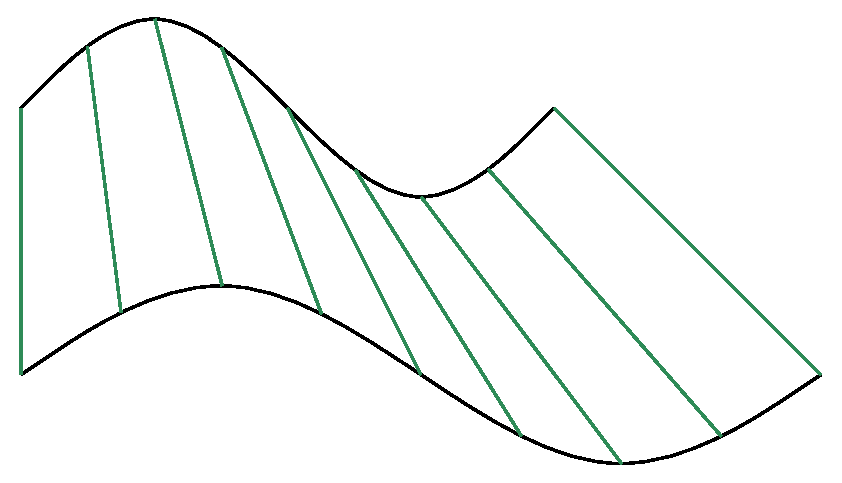
\includegraphics[width=\textwidth]{figures/dtw-stretch.eps}
                % \caption{HMM1}
                \label{fig:hmm1}
        \end{subfigure}%
        \quad
        \begin{subfigure}[b]{0.45\textwidth}
                \centering
                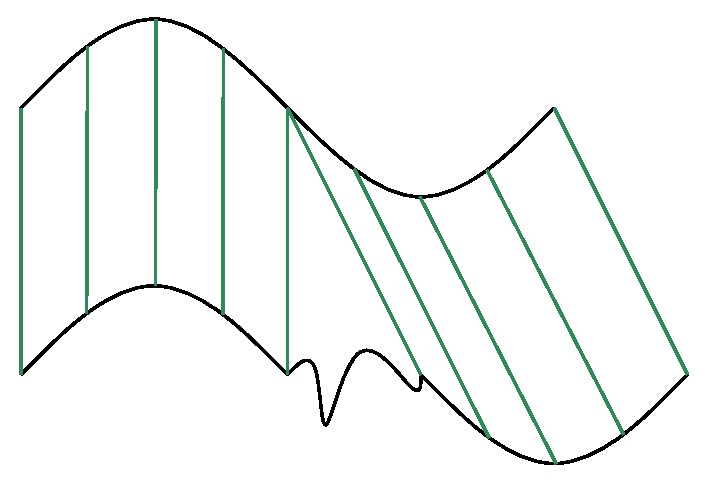
\includegraphics[width=\textwidth]{figures/dtw-distort.eps}
                % \caption{HMM1}
                \label{fig:hmm1}
        \end{subfigure}%

        \caption{DTW allows to match two time series even if they are stretched (left) or distorted (right) }
        \label{fig:dtw-model}
\end{figure}



Dynamic Time Warping is a dynamic programming algorithm to measure the similarity between two time series which may vary in time or speed. This has been used for speech recognition and can also be used for signature detection to cope with the non-linear time distortions which one might see in the signals because a signer does not always sign with the same speed. It has shown to be a much more robust distance measure than the Euclidean distance \cite{Keogh:2000:SUD:347090.347153}\cite{1030918}\cite{1227706} due to it's ability to match similar shapes even if they are out of phase in the time axis.

Koegh et al. showed on a very large dataset that the mean error rate average over 1000 runs for DTW was an order of magnitude lower than the error rate for the Euclidian distance. However, the DTW algorithm also took approximately 230 times longer than the Euclidean distance. \cite{Keogh:2002:EID:1287369.1287405}

It has first been applied to signatures in 1977 by Yasuhara and Oka \cite{yasuhara1977DTW} who concluded that is a very useful approach for online real-time signature verification. Yasuhara and Oka used an adaption of the algorithm that was originally poposed by Sakoe and Chiba \cite{1163055}.

DTW allows us to compare signatures even if the signer was signing slower at the beginning in one of the two signatures.

\textbf{Training} is done by computing the distance measure $dtw[n][m]$ for all signatures $n, m$ in the set of signatures for a certain user and selecting the signature $s$ with the smallest distance to all other signatures.

\textbf{Classification} is done by computing the distance DTW distance $dtw[s][t]$ between the model signature $s$ and a test signature $t$.

\textbf{Algorithm} We have two Signatures $X,Y$ defined as follows:

$$X = x_1, x_2, ... , x_i, ... , x_I$$ $$Y = y_1, y_2, ..., y_j, ..., y_J$$

and a distance measure defined as $$d(i,j) = ||x_i - y_i||$$

We define a warping path $C$ as $$ C = c_1, c_2, ..., c_k, ..., c_K $$ where each element $c_k$ correspondes to a combination $(x_i, y_i)$.

The algorithm is initialized with $$g_1 = g(1,1) = d(1,1) * w(1)$$ where $g_k$ is the accumulated distance after $k$ steps and $w(k)$ is a weighting function that has to be defined.
In each iteration, $g_k$ is computed as $$g_k = g(i,j) = \min\limits_{c_{k-1}} [g_{k-1}+d(c_k) * w(k)]$$ until both Signatures $X,Y$ have been traversed.

The normalized distance of the two signatures is therefore: $$D(X,Y) = \frac{g_K}{\sum_{k=1}^K w(k)}$$ where $\sum w(k)$ compensates the effect of the length of the sequences.

The definitionen of weighting factors $w_k$ defines the matching between the two signatures. The most common definitionen in literature is such that only three types of transitions - deletion, instertion and match - are allowed. The resulting $g_k$ becomes: $$g_k = g(i,j) = \min \left[\begin{array}{c}g(i,j-1) + d(i,j) \\g(i-1,j-1)+ 2 d(i,j) \\g(i-1,j) + d(i,j)\end{array}\right]$$


TODO: show image like 10.1007 s10115 page 362

Even though the DTW algorithm has been outperformed by more powerful algorithms like HMMs or SVMs in speech detection, it remains very effective in Signature detection as it deals well with small amounts of training data, which is typical for signature verification problems.

In general, DTW is known to have two drawbacks in signature verification:
\begin{itemize}
\item heavy computational load
\item warping of forgeries
\end{itemize}

DTW causes heavy computational load becauseit does not obey the triangular inequality and thus indexing a set of signatures takes a lot of time. As soon as the pool of signatures for a signer get bigger, the computation costs raise because the test signature has to be compared to each of the signatures in the pool of confirmed signatures. Eamonn Keogh et al. presented a lower bounding method to index all samples without comparing each of them to each other. \cite{Keogh:2002:EID:1287369.1287405}

The second drawback can be addressed by looking at how straight or bended the warping path is. A straight warping path indicates that a genuine signature is more likely whereas a curvy warping path indicates a forgery. Work on this has been done \cite{Sato1982} but made comparison between different signatures harder because it introduce another dimension and thus made computation harder and has hence not found wide spread use.

Hao Feng et al. proposed another extension of the DTW algorithm, called extreme points warping (EPW) which proved to be more adaptive in the field of signature verification than DTW and reduced the computation time by a factor of 11. \cite{Feng:2003:OSV:961320.961331} Instead of warping the signature as a whole, they only warp so called Extreme Points that are characteristic to a signer's signature and match the curves between those points linearly.



% Dynamic time warping is a classic dynamic programming algorithm that is also used in speech recognition.

% A signature verification system using DTW is reported by Martens and Clae- sen [14]. DTW is a method to measure the similarity between two sequences which may vary in time or speed. This similarity measure can be used to perform signature verification. Comparing two sequences can be done in many different ways such as correlation, integration of the difference of two signals etc. However all these similarity measures cannot cope with non-linear time distortions which we will have in the signature signals. If a user takes a little longer for the first letter of the signature, the similarity measure should not deteriorate more than if the user was taking a little longer on the last letter. The DTW method allows us to compare two signatures while a small time distortion in the beginning of the signature does not accumulatively deteriorate the similarity measure throughout the whole signature.

% page 10-12

% DTW Signature Verification

% Training the DTW signature verification algorithm is performed by calculating the distance measure (dtw[n][m]) for all pairs of signatures in the training set. The signature with the smallest mean distance measure to all the other signatures is selected as the prototypical signature of the given user.
% The DTW matching score of a signature to be verified is equal to the distance measure dtw[n][m] between the prototypical signature found during training and the signature under test.


% ==
% Although the DTW algorithm has been replaced by more powerful ones such as HMMs or SVMs for speech applications, it remains as a highly effective



\subsection{Hidden Markov models}

% Hidden Markov Models (HMM) have been widely used by the speech recognition community (Ra- biner, 1989) as well as in many handwriting recognition applications (Dolfing, 1998). Sev- eral approaches using HMMs for dynamic signature verification have been proposed in the last years (Dolfing et al., 1998; Fierrez et al., 2007; Muramatsu and Matsumoto, 2003; Van et al., 2007; Yang et al., 1995). An HMM represents a double stochastic process, governed by an underlying Markov chain, with a finite number of states and random function set that gen- erate symbols or observations each of which is associated with one state (Yang et al., 1995). Observations are modeled with GMMs in most speech and handwriting recognition applica- tions. GMMs, which can be considered a single-state HMM, have been also successfully used for signature verification (Richiardi and Drygajlo, 2003).

A Hidden Markov Model (HMM) is a stochastic process with an underlying Markov Model of which the states can not directly be observed but the only observations can be made. Each state transition emits a certain observation with a certain probability.

Other than with a Markov Model, the states of a Hidden Markov Model can not directly be observed. Only Symbols, which are emitted from each state with a certain probability, can be observeed.



Markov Models can be modeled as Left-to-right, ... (TODO: name all types, show graph).


\begin{figure}
        \centering
        \begin{subfigure}[b]{0.45\textwidth}
                \centering
                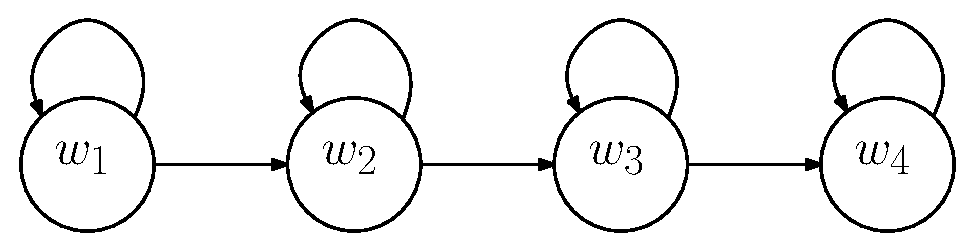
\includegraphics[width=\textwidth]{figures/hmm-ltr1.eps}
                % \caption{HMM1}
                \label{fig:hmm1}
        \end{subfigure}%
        \quad
        \begin{subfigure}[b]{0.45\textwidth}
                \centering
                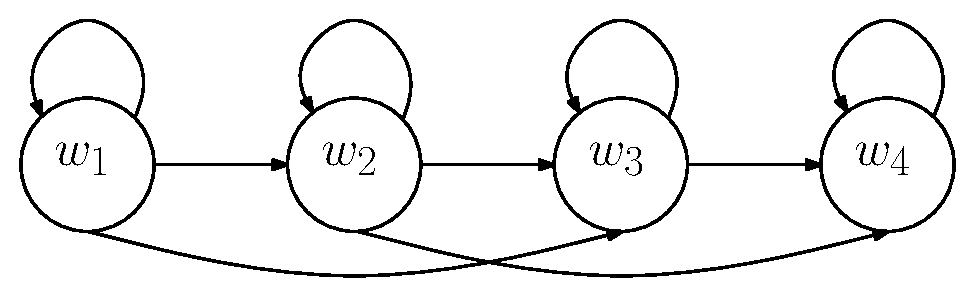
\includegraphics[width=\textwidth]{figures/hmm-ltr2.eps}
                % \caption{HMM1}
                \label{fig:hmm1}
        \end{subfigure}%

        ~ %add desired spacing between images, e. g. ~, \quad, \qquad etc.
          %(or a blank line to force the subfigure onto a new line)
        \begin{subfigure}[b]{0.45\textwidth}
                \centering
                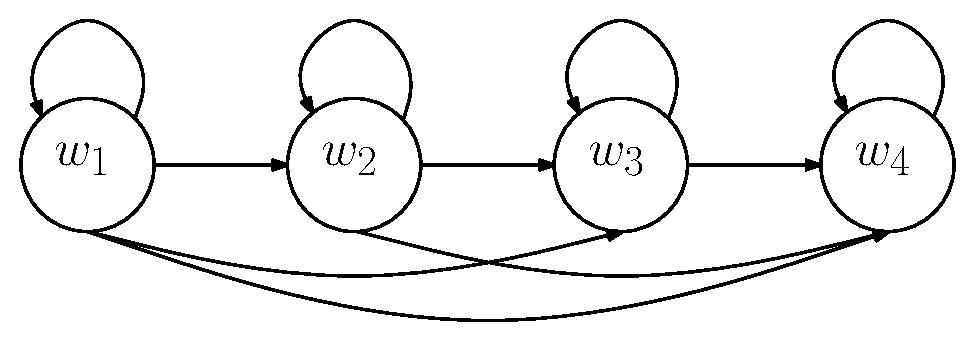
\includegraphics[width=\textwidth]{figures/hmm-ltr3.eps}
                % \caption{HMM1}
                \label{fig:hmm1}
        \end{subfigure}%
        \quad
        \begin{subfigure}[b]{0.45\textwidth}
                \centering
                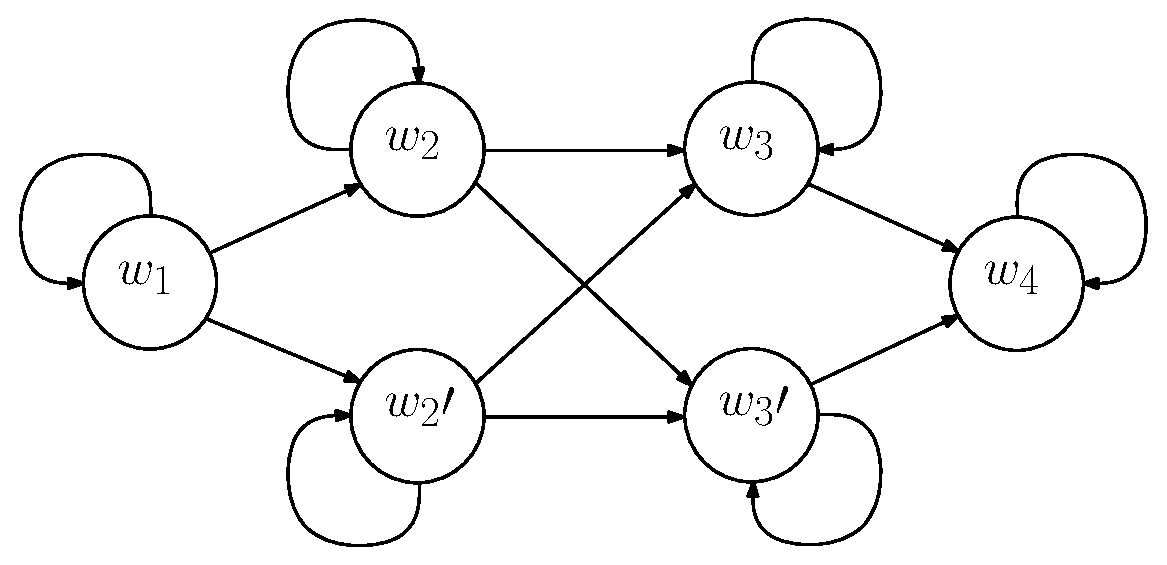
\includegraphics[width=\textwidth]{figures/hmm-ltr5.eps}
                % \caption{HMM1}
                \label{fig:hmm1}
        \end{subfigure}%

        \begin{subfigure}[b]{0.30\textwidth}
                \centering
                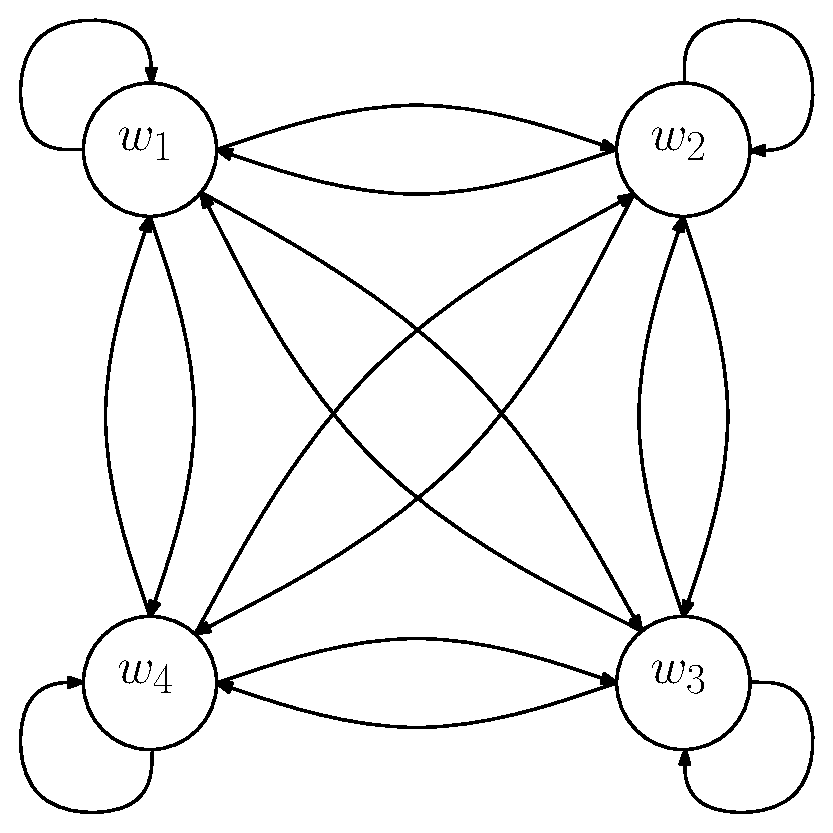
\includegraphics[width=\textwidth]{figures/hmm-ltr4.eps}
                % \caption{HMM1}
                \label{fig:hmm1}
        \end{subfigure}%



        \caption{Different Markov Models: a: ...}\label{fig:markov-models}
\end{figure}



While HMMs with a too small set of states and observations perform bad because they are too simple, too many states and observations make the model computational heavy and accuracy is reduced because of overfitting.

There are three fundamental problems for HMMs:
Given the model parameters and observed data, estimate the optimal sequence of hidden states.
Given the model parameters and observed data, calculate the likelihood of the data.
Given just the observed data, estimate the model parameters.
The first and the second problem can be solved by the dynamic programming algorithms known as the Viterbi algorithm and the Forward-Backward algorithm, respectively. The last one can be solved by an iterative Expectation-Maximization (EM) algorithm, known as the Baum-Welch algorithm.


Baum-Welch-Algorithm

\begin{figure}[tb]
    \begin{center}
        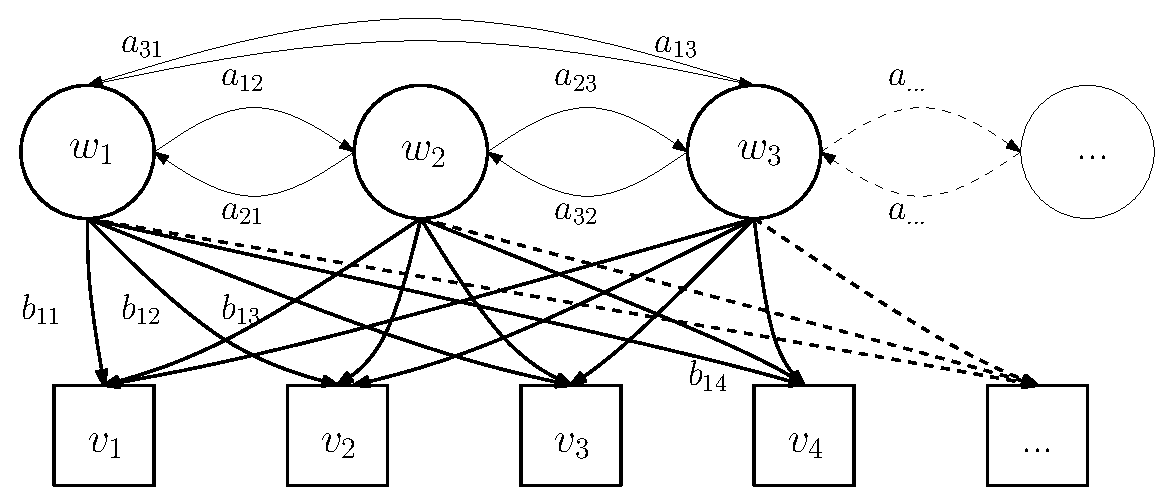
\includegraphics[width=\textwidth]{figures/hmm-general-model.eps}
    \end{center}
    \caption{General representation of an HMM with states $w_1, w_2, 2_3, ...$ and observations $v_1, v_2, v_3, ...$}
    \label{fig:hmm-general-model}
\end{figure}

\textbf{Algorithm}: An HMM is defined by the following elements:

The HMM consists of $N$ states $w_1, w_2, ..., w_N$, each of which cannot be directly observed. Each of the states emits a symbol at time $t$ which can be observed. Therefore, after going through $T$ time steps, the System emits the sequence $$V^T = \{ v(1), v(2), ..., v(T)\}$$

The probabilities to go from one state to another are given by the Transition matrix $A$ with elements $$a_{ij} = P(w_j(t+1)|w_i(t))$$

The probability that a system is a certain state when an certain symbol is observed, is defined by the emission matrix $B$ with elements
$$b_j(v(t)) = P(v(t)|w_j(t))$$

$A$ and $B$ fulfill the normalisation condition:
$$\sum_k b_j(k) = 1, \sum_{j=1}^{N} a_{ij} = 1$$


$\pi$ defines the initial probability distribution for a csystem to be in a certain state.

To summarize, an HMM is defined by the transition matrix $A$, the emission matrix $B$ and the initial distribution $\pi$.


Therefore,

\begin{itemize}
\item Number of (hidden) States: $N$
\item Number of Symbols per State: $M$
\item Probability transition matrix $A = \{a_{ij}\}$ which defines the probability of going from one state to any other state or itself and holds $\sum_{j=1}^{N} a_{ij} = 1$ for all states $i$
\end{itemize}



\textbf{Training}:






% Finding a reliable and robust model structure for dynamic signature verification is not a trivial task. While too simple HMMs may not allow to model properly the user signatures, too complex models may not be able to model future realizations due to overfitting. On the other hand, as simple models have less parameters to be estimated, their estimation may be more robust than for complex models.


% El-Yacoubi [17] uses HMMs and the cross-validation princi- ple for random forgery detection. A grid is superimposed on each signature image, segmenting it into local square cells. From each cell, the pixel density is computed so that each pixel density represents a local feature. Each signature im- age is therefore represented by a sequence of feature vectors, where each feature vector represents the pixel densities asso- ciated with a column of cells. The cross-validation principle involves the use of a subset (validation set) of each writer’s training set for validation purposes. Since this system aims to detect only random forgeries, subsets of other writers’ train- ing sets are used for impostor validation. Two experiments are conducted on two independent data sets, where each data set contains the signatures of 40 and 60 writers, respectively. Both experiments use 20 genuine signatures for training and 10 for validation. Both experiments use the forgeries of the first experiment for impostor validation. Each test signature is analyzed under several resolutions and the majority-vote rule is used to make a decision. AERs of 0.46% and 0.91% are reported for the respective data sets.
% Justino [18] uses a discrete observation HMM to detect random, casual, and skilled forgeries. A grid segmentation scheme is used to extract three features: a pixel density fea- ture, a pixel distribution feature (extended-shadow-code), and an axial slant feature. A cross-validation procedure is used to dynamically define the optimal number of states for each model (writer). Two data sets are used. The first data set contains the signatures of 40 writers with 40 genuine signa- tures per writer. This data set is used to determine the opti- mal codebook size for detecting random forgeries. This op- timised system is then used to detect random, casual, and skilled forgeries in a second data set. The second data set contains the signatures of 60 writers with 40 training signa- tures, 10 genuine test signatures, 10 casual forgeries, and 10 skilled forgeries per writer. An FRR of 2.83% and an FAR of 1.44%, 2.50%, and 22.67% are reported for random, casual, and skilled forgeries, respectively.



% \subsection{Neural networks}

% Neural networks have also been used to build a system for detection of random forgeries. (TODO: explain random forgeries, list reference Baltzakis)
% Baltzakis uses global features, grid features such as pixel densities and texture features such as cooccurrence matrices to represent each signature. A two-stage perceptron one-class-one-network (OCON) calssification is used for each feature set.
% TODO: explain more when reference found



% Baltzakis [16] developed a neural network-based system for the detection of random forgeries. The system uses global features, grid features (pixel densities), and texture features (cooccurrence matrices) to represent each signature. For each one of these feature sets, a special two-stage percep- tron one-class-one-network (OCON) classification structure is implemented. In the first stage, the classifier combines the decision results of the neural networks and the Euclidean dis- tance obtained using the three feature sets. The results of the first stage classifier feed a second-stage radial basis function (RBF) neural network structure, which makes the final de- cision. A database is used which contains the signatures of 115 writers, with between 15 and 20 genuine signatures per writer. An average FRR and FAR of 3% and 9.8%, respectively is obtained.
% Kaewkongka [8] uses the Hough transform (general Radon transform) to extract the parameterised Hough space from a signature skeleton as a unique characteristic feature of a signature. A backpropagation neural network is used to evaluate the performance of the method. The system is tested with 70 signatures from different writers and a recognition rate of 95.24% is achieved.
% Quek [13] investigates the feasibility of using a pseudo- outer product-based fuzzy neural network for skilled forgery detection. He uses global baseline features (i.e., the vertical and horizontal position in the signature image which corre- sponds to the peak in the frequency histogram of the vertical and horizontal projection of the binary image, respectively), pressure features (that correspond to high pressure regions in the signature), and slant features (which are found by ex- amining the neighbours of each pixel of the thinned signa- ture). He then conducts two types of experiments. The first group of experiments use genuine signatures and forgeries as training data, while the second group of experiments use only genuine signatures as training data. These experiments are conducted on the signatures of 15 different writers, that is, 5 writers from 3 different ethnic groups. For each writer, 5 genuine signatures and 5 skilled forgeries are submitted. When genuine signatures and forgeries are used as training data, the average of the individual EERs is 22.4%. Compa- rable results are obtained when only genuine signatures are used as training data.




% \subsection{Template matching techniques}

% Deng [7] developed a system that uses a closed contour trac- ing algorithm to represent the edges of each signature with several closed contours. The curvature data of the traced closed contours are decomposed into multiresolutional sig- nals using wavelet transforms. The zero crossings corre- sponding to the curvature data are extracted as features for matching. A statistical measurement is devised to decide sys- tematically which closed contours and their associated fre- quency data are most stable and discriminating. Based on these data, the optimal threshold value which controls the ac- curacy of the feature extraction process is calculated. Match- ing is done through dynamic time warping. Experiments are conducted independently on two data sets, one consisting of English signatures and the other consisting of Chinese sig- natures. For each experiment, twenty-five writers are used with ten training signatures, ten genuine test signatures, ten skilled forgeries, and ten casual forgeries per writer. When only the skilled forgeries are considered, AERs of 13.4% and 9.8% are reported for the respective data sets. When only the casual forgeries are considered, AERs of 2.8% and 3.0% are reported.
% Fang [9] proposes two methods for the detection of skilled forgeries. These methods are evaluated on a database of 1320 genuine signatures from 55 writers and 1320 forg- eries from 12 forgers. In determining the FRR, the leave- one-out method was adopted to maximise the use of the available genuine signatures. The first method calculates one- dimensional projection profiles for each signature in both the horizontal and vertical directions. These profiles are then op- timally matched with reference profiles using dynamic pro- gramming. This method differs from previous methods in the sense that the distance between the warped projection profiles is not used in the decision. Instead, the positional distortion of each point of the sample profile, when warped onto a reference profile, is incorporated into a distance mea- sure. A Mahalanobis distance is used instead of a simple Euclidean distance. The leave-one-out covariance (LOOC) method is adopted for this purpose, but the unreliable off- diagonal elements of the covariance matrices are set to zero. When binary and gray-scale signatures are considered, the best AERs for this method are 20.8% and 18.1%, respectively. The second method matches the individual stroke segments of a two-dimensional test signature directly with those of a template signature using a two-dimensional elastic match- ing algorithm. The objective of this algorithm is to achieve maximum similarity between the “elements” of a test signa- ture and the “elements” of a reference signature, while min- imising the deformation of these signatures. A gradient de- scent procedure is used for this purpose. Elements are short straight lines that approximate the skeleton of a signature. A
% Mahalanobis distance with the same restrictions as for the first method is used. An AER of 23.4% is achieved for this method.
% Guo [11] approached the offline problem by establish- ing a local correspondence between a model and a ques- tioned signature. The questioned signature is segmented into consecutive stroke segments that are matched to the stroke segments of the model. The cost of the match is deter- mined by comparing a set of geometric properties of the corresponding substrokes and computing a weighted sum of the property value differences. The least invariant fea- tures of the least invariant substrokes are given the largest weights, thus emphasizing features that are highly writer de- pendant. Using the local correspondence between the model and a questioned signature, the writer dependant informa- tion embedded at the substroke level is examined and un- ballistic motion and tremor information in each stroke seg- ment are examined. Matching is done through dynamic time warping. A database with 10 writers is used with 5 train- ing signatures, 5 genuine test signatures, 20 skilled forgeries, and ten casual forgeries per writer. An AER of 8.8% is ob- tained when only skilled forgeries are considered and an AER of 2.7% is obtained when only casual forgeries are consid- ered.


% \subsection{Minimum distance classifiers}

% Fang [10] developed a system that is based on the assump- tion that the cursive segments of forged signatures are gener- ally less smooth than that of genuine ones. Two approaches are proposed to extract the smoothness feature: a crossing method and a fractal dimension method. The smoothness feature is then combined with global shape features. Verifi- cation is based on a minimum distance classifier. An itera- tive leave-one-out method is used for training and for testing genuine test signatures. A database with 55 writers is used with 24 training signatures and 24 skilled forgeries per writer. An AER of 17.3% is obtained.
% Fang [14] also developed a system that uses an elastic matching method to generate additional samples. A set of peripheral features, which is useful in describing both the in- ternal and the external structures of signatures, is employed to represent a signature in the verification process. Verifica- tion is based on a Mahalanobis distance classifier. An itera- tive leave-one-out method is used for training and for test- ing genuine test signatures. The same database that was used in Fang’s previous paper [10] is again used here. The addi- tional samples generated by this method reduced the AER from 15.6% to 11.4%.
% Mizukami [15] proposed a system that is based on a dis- placement extraction method. The optimum displacement functions are extracted for any pair of signatures using min- imization of a functional. The functional is defined as the sum of the squared Euclidean distance between two signa- tures and a penalty term that requires smoothness of the displacement function. A coarse-to-fine search method is applied to prevent the calculation from stopping at local minima. Based on the obtained displacement function, the
% Offline Signature Verification Using the DRT and a HMM
% 563
% dissimilarity between the questioned signature and the cor- responding authentic one is measured. A database with 20 writers is used with 10 training signatures, 10 genuine test signatures, and 10 skilled forgeries per writer. An AER of 24.9% is obtained.
% Sabourin [12] uses granulometric size distributions for the definition of local shape descriptors in an attempt to characterise the amount of signal activity exciting each retina on the focus of an superimposed grid. He then uses a nearest neighbour and threshold-based classifier to detect random forgeries. A total error rate of 0.02% and 1.0% is reported for the respective classifiers. A database of 800 genuine sig- natures from 20 writers is used.





% \section{Online Signature Detection}
% % Online signature verification methods are generally categorized to either use global or local features to classify a given signature

% % ==

% % On-line or dynamic systems use captured signature time-functions. These functions are obtained using digitizer tablets or touchscreens (e.g. Tablet-PCs, smart phones, etc.). Tradition- ally, dynamic systems have presented a better performance than off-line systems as more levels of information than the signature static image are available (Plamondon and Lorette, 1989). This is the approach considered in this work, and will be described in the following chapters.

% % Feature Extraction: Two main approaches have been followed in this step: feature- based systems extract global features (e.g. signature duration, number of pen-ups, average velocity) from the signature in order to obtain a holistic feature vector (Lee et al., 1996). On the other hand, function-based systems use the signature time functions (e.g. position, pressure) for verification. Traditionally, function-based approaches have yielded better results than feature-based ones (Fierrez-Aguilar et al., 2005a; Kholmatov and Yanikoglu,
% 2005).


% \subsection{Feature-Based Methods}
% % As the name suggests, feature-based methods use features extracted from the sig- natures to perform the verification task. In general two different types of features are considered: global and local. Global features are related to the signature as a whole, for instance the signature duration or the mean pressure applied. Local features are based on single sample points. Examples for local features are the maximum velocity or the highest curvature.

% % Lee et al. [5].

% % A large number of features useful for signature verification was listed by Fierrez-Aguilar et al. [6].

% % This is why in general a smaller set of more discriminative features is preferred. The issue of feature selection in the signature verification task was extensively studied by Richiardi et al. [7].

% % After having found a suitable feature vector, an arbitrary one-class classifi- cation scheme can be used to perform the classification into valid and invalid signatures. Since there is no negative training data available, the task of classifi- cation is very similar to the task of outlier- or novelty detection. Several methods to perform such a classification are known [8].




% \subsection{Function-Based Methods}

% % Function-based signature verification methods are focused on building a signa- ture model which accurately reflects the temporal behaviour of the signature. Instead of extracting features that are used for verification, the emphasis of the signature model lies in the (timed) sequence of strokes drawn during the signing process. Comparing any signature to the model built during training will lead to a match score which is based on the level of similarity between (timed) sequence of strokes in the model and the signature under test. Function-based methods are reported to deliver better performance than global feature based methods [6]. Two function-based methods are predominant in the literature: Hidden Markov Model based methods and Dynamic Time Warping (DTW) based methods.

% % page 6-8 for sample feature set

% % Function-based methods to perform signature verification compare the tempo- ral behaviour of the recorded signals x(t), y(t), p(t) and a(t). In this work, a dynamic time warping based method is used. The performance of a Hidden Markov Model system might be higher than the DTW system performance but the implementation complexity is much lower for the DTW system.







\section{Challenges in Signature Detection Specific to Mobile Payments}

A lot of work has been done on signature detection on static signatures and also on dynamic signatures. However, almost all work on dynamic signatures has been done on signatures that were captured using a pen on a digital tablet. In our case, signatures were captured on a wide range of different devices and with a user's finger instead of a pen. This has several implications.

Our experiments in chapter X (TODO ref) will show to which extent known techniques are applicable to this type of signature and what future work might need to be done.

\subsection{Signature are written with Finger}

Our experience shows that people are not used to write their signature with their bare finger and the first few times they sign, their signature differs a lot. However, after just 10-15 times , the signature's shape seems to stabilize.

This means that it will be a lot harder to detect signatures based on the first few signatures than on later signatures, once a user got used to signing with her finger.

It also means that we should prefer later signatures to earlier ones as in later signatures the signer's signature might have stabilized.


\subsection{Sparse Initial Dataset}

Although SumUp is live in over 10 countries as of today, it is still only used in a relatively small set of locations and we are therefore unlikely to gather a lot of data about a certain user until the concept becomes more often deployed and used.

This means that we have to try and find a solution that works reasonably well with a small amount of initial data per user.


\subsection{Device \& Software Fragmentation}

Unlike the signature's that are captured on a digital tablet, our database of signatures is captured on a variety of devices with different properties. There are various factors that have an influence on the digital representation of the signature:

\begin{itemize}
\item Different Manufacturer: Both, iOS and Android devices use a variety of manufacturers for their handsets and the touch screens used. Recent studies have shown the differences of how signals are captured on different screens (TODO: link reference)
\item Screen Size: the screen diagonal of current smartphones typically ranges between X and X cm, those of tablets typically ranges between X and X cm. A consequence is that the user might not only sign slightly differently but also that the signature will consist of more or less data points and it will take users a longer or shorter amount of time to sign.
\item  ...
\end{itemize}


We will consider these factors when applying our algorithm in Chapter X (TODO)


\section{Feedback Loop}




















%%%%%%%%%%%%%%%%%%%%%%%%%%%%%%%%%%%%%%%% CHAPTER EXPERIMENTS
\chapter{Experiments}
\label{chp:experiments}
% offline vs online
% using dynamic features: speed, acceleration


% Circle Detection?
% X Detection?

Section \ref{sec:exp-preventive} will give insight into how our work has affected the number of false positives and thus the manual inputs from Operations have changed since the new component was released.

Section \ref{sec:exp-reactive} will first introduce the database of signatures we collected to test our signature verification algorithms and afterwards show the equal error rate (EER) achieved in different scenarios.


\section{Preventive Fraud Detection}
\label{sec:exp-preventive}

The algorithms described in Listing \ref{lst:world-check-parse} and Listing \ref{lst:world-check-lookup} were implemented in a Ruby Sinatra app with a REST interface and released to production about 2 months prior to the submission of this thesis.

\subsection{Setup}

The full database was parsed on a testing environment and the resulting data was copied over into production. The daily updates are received on the production machine and directly parsed into the production database through the parsing script.

The PEP/HRA check is performed either automatically or manually:
\begin{itemize}
\item \textbf{Automatically} for each new user during sign-up
\item \textbf{Automatically} for each existing user once a week to re-check each account after incorporating the changes of that week
\item \textbf{Manually} from the Operations Admin Panel (OAP) via a button
\end{itemize}

Each request must be triggered via a POST request. Depending on the user object that needs to be checked, the body of the request changes. Table \ref{tbl:har-pep-requests} lists the different request types.

\begin{table}[tb]
    \begin{center}
        \begin{tabular}{p{1.75cm}|p{3cm}p{7cm}}
        \hline
        \textbf{Method} & \textbf{Path} & \textbf{Parameter} \\
        \hline
        POST & /person/check & \{"params": \{"user\_id": "1"\}\} \\ \hdashline[0.5pt/3pt]
        POST & /person/check & \{"params": \{"business\_owner\_id": "1"\}\} \\ \hdashline[0.5pt/3pt]
        POST & /person/check & \{"params": \{"business\_officer\_id": "1"\}\} \\
        \hline
        \end{tabular}
    \end{center}
    \label{tbl:har-pep-requests}
    \caption{The requests received by the PEP/HAR component}
\end{table}

\subsection{Results}

Show how many false positives/false negatives were collected before switch to new component and after switch.




\section{Reactive Fraud Detection}
\label{sec:exp-reactive}

\subsection{Database}

As there don't seem to be any publicly available databases of signatures that were collected with a finger on a mobile device, we collected our own database and forgeries.

Between 8 and 80 Signatures per person were collected from 11 people on 4 different days on four different devices. In total, a set of 487 signatures was collected.

The devices used to collect the signatures are listed in Table \ref{tbl:signatures-devices}.

\begin{table}[tb]
    \begin{center}
        \begin{tabular}{p{1.75cm}|p{2cm}p{2cm}p{2cm}p{2cm}}
        \hline

        \hline
        \textbf{Device} & \textbf{Software Version} & \textbf{Screen Size [cm]} & \textbf{Screen Resolution [px]} & \textbf{Pixel Density [ppi]} \\
        \hline
        Apple iPhone 4s & iOS 6.1.2 & 8.9 & 640x960 & 326 \\
        \hdashline[0.5pt/3pt]
        Apple iPhone 5 & iOS 6.1.2 & 10 & 640x1136 & 326 \\
        \hdashline[0.5pt/3pt]
        Samsung Galaxy Note II & Android 4.1.1 & 14.1 & 720x1280 & 267 \\
        \hdashline[0.5pt/3pt]
        Apple iPad mini & iOS 6.1.2 & 20 & 768x1024 & 163\\
        \hline
        \end{tabular}
    \end{center}
    \label{tbl:signatures-devices}
    \caption{The four devices used to collect signatures, ordered by screen size}
\end{table}

We also collected three forgeries for each person. The forgeries were created by an untrained person in the following modi.

\begin{itemize}
\item \textbf{Spontaneous Forgery}: A random signature from the set of one person's signatures was shown the imposter for 5 secs. The imposter was only allowed to forge the signature after the five seconds.
\item \textbf{Sample Forgery}: A random signature from the set of one person's signatures was shown to the imposter for an indefinite amount of time and the imposter was able to look at the signature while forging the signature.
\item \textbf{Knowledgable Forgery}: The imposter had unlimited access to all of one person's signatures to forge the signature.
\end{itemize}

\subsubsection{Pre-Alignment and Normalization}

% \section{Databases}
% most available signature DB are pen/tablet signatures


\subsection{Forgeries}
% A signature verification system typically focuses on the detection of one or more category of forged signatures. A skilled forgery is produced when the forger has unrestricted
% access to one or more samples of the writer’s actual signa- ture (see Figure 1b). A casual forgery or a simple forgery (see Figure 1c) is produced when the forger is familiar with the writer’s name, but does not have access to a sample of the ac- tual signature—stylistic differences are therefore prevalent. A random forgery or zero-effort forgery (see Figure 1d) can be any random scribble or a signature of another writer, and may even include the forger’s own signature. The genuine signatures and high quality forgeries for other writers are usually considered to be forgeries of this type.
% Skilled forgeries can be subdivided into amateur and pro- fessional forgeries. A professional forgery is produced by an in- dividual who has professional expertise in handwriting anal- ysis. They are able to circumvent obvious problems and ex- ploit their knowledge to produce high-quality, spacial forg- eries (see Figure 2b).

% In the context of online verification, amateur forgeries can be subdivided into home-improved and over-the-shoulder forgeries (see [6]). The category of home-improved forgeries contains forgeries that are produced when the forger has a paper copy of a genuine signature and has ample opportu- nity to practice the signature at home. Here the imitation is based only on the static image of the original signature (see Figure 2c). The category of over-the-shoulder forgeries contains forgeries that are produced immediately after the forger has witnessed a genuine signature being produced. The forger therefore learns not only the spatial image, but also the dynamic properties of the signature by observing the signing process (see Figure 2d). The different types of forg- eries are summarised in Figure 3.


% Three types of forgeries were considered: ”over the shoulder” (O.S.), ”home improved” (H.I.) and ”professional” (PR.). The first kind of forgeries (O.S.) were captured by the forger after he has seen the gen- uine signature being written, that is after knowing the dy- namic properties of the signature by observation of the sign- ing process. Of course, in this case, the forger also learns the spatial image of the signature. The second type of forg- eries (H.I.) are made in other conditions: the forger only imitates the static image of the genuine signature, and has the possibility of practicing the signature at home. Finally, the last kind of forgeries (PR.) are produced by individu- als who have professional expertise in handwriting analy- sis. They exploit their experience in discriminating gen- uine from forged signatures to produce high quality spatial forgeries. This database contains 1530 genuine signatures, 1470 O.S. forgeries (30 per individual except two), 1530 H.I. forgeries (30 per individual), and 200 PR. forgeries (10 per individual for 20 individuals).


% \subsection{SumUp}


% \subsection{SVC2004}
% Two development databases were released prior to the Signature Ver- ification Competition (SVC) 2004 (Yeung et al., 2004). They were captured using a WACOM digitizing tablet and a Grip Pen. Due to privacy issues, users were advised to use invented signatures as genuine ones. The two databases differ in the available data, and correspond to the two tasks defined in the competition. One contains only coordinate information while the other provides also pressure and pen orientation signals. Each database contains 40 users, with 20 genuine signatures and 20 forgeries per user acquired in two sessions. Both occidental and asian signatures are present in the databases. Examples of signatures from this database are shown in Fig. 2.6.

% \subsection{SUSig}


% \subsection{ATVS-SSig\_DB}

% \section{Experimental Setup}

% \section{Feature Selection}
% ==
% Due to the curse of dimensionality (Theodoridis and Koutroumbas, 2006), the performance of a statistical classifier is degraded if the available training data is too small compared to the number of dimensions of the feature vector (Jain and Zongker, 1997). This is usually the case in signature verification, where the average length of a digitized signature is of a few hundreds of samples and the available number of training signatures is relatively small (in practical applications between 3 and 5). The amount of training signatures is mostly conditioned by the willingness of the users to provide many samples during enrollment. Nevertheless, when signatures are captured during only one unique session, their variability is small in general, leading to a poorly trained model.
% Feature selection techniques try to reduce the dimensionality of the feature vectors while optimizing the verification accuracy. Their goal is to find the optimum combination of features according to a given optimization criterion. Ideally, given a feature vector of F dimensions, all the possible combinations from 1 to F features should be tested in order to find the optimal combination.
% p15++



\subsection{Experiment Setup}

\subsubsection{Feature Extraction}

% From 01030918.pdf:
% Like in [2], in order to estimate the speed at time 􏰥, we consider the point visited at time 􏰥, 􏰖 􏰶􏰥􏰷 􏰭 􏰶􏰨􏰶􏰥􏰷􏰈 􏰩 􏰶􏰥􏰷􏰷 and its two neighbors in the se-
% quence (see Fig. 1), that is 􏰖 􏰶􏰥 􏰰 􏰫􏰷 and 􏰖 􏰶􏰥 􏰸 􏰫􏰷. We
% estimate the speed in the 􏰨 and 􏰩 directions respectively by
% 􏰦􏰨􏰶􏰥􏰷 􏰭 Æ􏰨􏰶􏰥􏰷 􏰭 􏰨􏰶􏰥 􏰸 􏰫􏰷 􏰰 􏰨􏰶􏰥 􏰰 􏰫􏰷 and􏰦􏰩􏰶􏰥􏰷 􏰭 Æ􏰩􏰶􏰥􏰷 􏰭
% 􏰩 􏰶􏰥 􏰸 􏰫􏰷 􏰰 􏰩 􏰶􏰥 􏰰 􏰫􏰷, and so an estimate of speed magni- 􏱈
% tudeattime􏰥 isgivenby􏱇􏱇􏰦 􏰶􏰥􏰷􏱇􏱇 􏰭 Æ 􏰨􏰶􏰥􏰷 􏰬 􏰸 Æ 􏰩
% include also for motion direction 􏰂􏰶􏰥􏰷 and Æ 􏰂􏰶􏰥􏰷 under the form of their cosine and sine.1 Besides these 5 dynamic features, we keep the axial pressure and the pen-tilt. Fur- thermore, following the principle in [11], we extract a low resolution image (of 9 values) around each point in order to introduce spatial information. As shown in Fig. 1, a 􏰺 􏰱 􏰺 window centered on each point of this sequence permits to compute a ”context bitmap” as follows: when the window is centered on a pen-down, the number of pen-down points in each of the 9 rectangles are computed; when the win- dow is centered on a pen-up, the 9 values representing the low resolution image of spatial context are all set to zero. This permits to introduce rough variations in such parame- ters when a pen-up appears in the sequence. The window shifts along the trajectory described by the pen, point per point. Therefore, 17 parameters are extracted on each point of the sequence: 8 dynamic and 9 static.


\subsubsection{Dynamic Time Warping}


\subsubsection{Hidden Markov Models}

list different packages that are available and why we chose to work with matlab

\subsubsection{Model}

% We chose a discrete HMM to model each signer’s charac- teristics [15]. This avoids making assumptions on the form of the underlying distribution, specially when there is not much data as it is the case in signature verification. A sig- nature is modeled by a left-to-right HMM in order to take into account the regularities appearing in the sequence rep- resenting a signature. The number of states in each signer’s HMM is between 6 and 12, depending on the average length of his signature. The topology only authorizes transitions between each state to itself and to its immediate right-hand neighbors. The K-Means algorithm is used during training to create a codebook of 100 centers for each signer. This was judged a good trade-off between the number of cen- ters describing the space of the signer, and the number of observation vectors collected in the training database of the signer, corresponding to 15 signatures. By means of the Nearest Neighbors rule, each signature is encoded as a se- quence of symbols, that are the centers of the signer’s space.

\subsubsection{Training}
% For each signer 􏰠, HMM learning is done only on genuine signatures of 􏰐 􏰠􏰫 (15 signatures). The Baum-Welch algo- rithm was used during training


\subsubsection{Evaluation/Matching}
% For each signer 􏰠, HMM learning is done only on genuine signatures of 􏰐 􏰠􏰫 (15 signatures). The Baum-Welch algo- rithm was used during training, and the Viterbi algorithm during the verification phase to approximate the likelihood of the signature given the model [15]. As done in previous works [4, 5, 7, 16], we have used the Viterbi log-likelihood score divided by the number of points in the signature in order to perform verification.


% As in [4], signature verification for signer 􏰠 was first per-formed using an adaptive threshold 􏰆 􏰮􏰞􏰮􏰣􏰥 􏰶􏰠􏰷 􏰭 􏰴􏰡 􏰶􏰠􏰷 􏰰 􏰨 where 􏰴􏰡 􏰶􏰠􏰷 denotes the average normalized log-likelihood score on the training database of signer 􏰠 and 􏰨 denotes an offset that is common to all signers. The decision is made on whether the pretended signature of signer 􏰠 is authentic or forged comparing the normalized log-likelihood score to this threshold. Two types of error are characteristic of the signature verification problem: false rejection (􏰏 􏰗 ), that is when an authentic signature is rejected, and false accep- tance (􏰏 􏰋), that is when a forgery is accepted. The level of these two error rates depends on the offset chosen; tradition- ally, the value of 􏰨 is chosen such as to realize the Equal Er- rorRate􏰎 􏰎 􏰗 (􏰏 􏰋 􏰭 􏰏 􏰗 ).Inordertoestimatetheoffset, we minimize the quadratic criterion 􏰶􏰏 􏰋􏰶􏰨􏰷 􏰰 􏰏 􏰗 􏰶􏰨􏰷􏰷 􏰬 on 􏰌 􏰋 (2330 signatures), which contains only genuine signa- tures and forgeries from signers of 􏰘 􏰫 (see Table 1). Then, we test the decision threshold on 􏰌 􏰙 (1365 signatures - same scheme for signers of 􏰘 􏰬 ).


% \subsection{MLP}
% http://en.wikipedia.org/wiki/Multilayer_perceptron

% In opposition to the sequential and generative approach characteristic of the HMM expert, we have privileged here, for more complementarity, a discriminating model based on global features. Table 4 presents these features. No pre- liminary filtering was necessary for computing these fea- tures because the noise effect was neglectable since they result of a summation over the entire signature. Vari- ables􏰦 􏰨 􏰈 􏰦􏰩 􏰈 􏰂􏰈 Æ 􏰂􏰈 􏰄􏰨 and􏰄 􏰩 havebeenpreviouslydefined in sections 3.1 and 3.2. The four histograms (parameters 11-26) of Table 4 count the angles (􏰂􏰈 Æ 􏰂􏰈 􏰄 􏰨 􏰈 􏰄􏰩 ) which be- long to quadrants 1,2,3,4. This choice of features seems to be discriminant, according to [6], even if the importance of a feature depends strongly on the signer. This number of features may seem important, but as we deal with a great number of signers we need several features to characterize the signers’ variability. Moreover, our learning procedure

% will allow a - specific to each signer - elimination of unnec- essary features.
% 4.2. The MLP training and testing phase
% We have designed one MLP expert for each signer. Due to the important number of MLPs, we have automated the training procedure: each MLP has 26 inputs, 5 hidden neu- ral units, and two sigmoidal outputs. Each training database consists in 15 genuine signatures and 15 ”other” signatures (􏰌 􏰋􏰔 , see Table 1) , because in real situations, the use of forgeries for training is not possible as they may not always be available. We train the MLP with a regularization tech- nique as described in [10], which reduces the complexity of the network and enables us to use small training-databases (30 examples). We have tested the networks on 􏰌 􏰙 and 􏰌 􏰙 􏰔 databases (see Table 1). As can be seen on Table 5, in both cases this network gives excellent performance for 􏰏 􏰗 rate, because MLPs manage to separate completely the class of the signer with the ”rest of the world”. On database 􏰌 􏰙 conversely, performance on forgeries are very poor, which was expected, because MLPs did not learn any forg- eries during the training phase. On 􏰌 􏰙 􏰔 database, perfor- mance on others (􏰕 􏰋 for Others Accepted) are better than forgeries on 􏰌 􏰙 , but not neglectable because we had too few examples (only 15) of ”other” signatures to build the separator between genuine signatures of a given signer and the ”rest of the world”. Note that in Table 5 no 􏰏 􏰋 rate is provided on 􏰌 􏰙 􏰔 which has no forgeries. Finally we have observed that the estimated effective number of param- eters [10] was always less than 40, which is less important than the initial 147 of each MLP expert.


\section{Evaluation}
% Throughout this paper, the false rejection rate (FRR), the false acceptance rate (FAR), the equal error rate (EER), and the average error rate (AER) are used as quality performance measures. The FRR is the ratio of the number of genuine test signatures rejected to the total number of genuine test sig- natures submitted. The FAR is the ratio of the number of forgeries accepted to the total number of forgeries submitted. When the decision threshold is altered so as to decrease the FRR, the FAR will invariably increase, and vice versa. When a certain threshold is selected, the FRR is equal to the FAR. This error rate is called the EER and the corresponding threshold may be called the equal error threshold. The average of the FRR and FAR is called the AER. When a threshold is used,

% that is, close to the equal error threshold, the FRR and FAR will not differ much. In this case the AER is approximately equal to the EER.


\subsection{Computational Requirements}
% An automatic signature verification system can only be eco- nomically viable when the processing requirements are feasi- ble. The practicality of our system as a real-time application depends on the number of floating point operations (flops) required to verify a test signature. The bulk of these flops are
% required to calculate the DRT. Much less flops are required to match a set of feature vectors (which represents a test signa- ture) with the HMM of the claimed writer’s signature.

% DRT
% We assume that the original image consists of Ψ pixels and that Θ angles (between 0◦ and 180◦) are used to calculate the DRT. When β (i.e., the number of beams per angle) is taken to be equal to the highest dimension of the original image, the number of flops required to calculate the DRT is on the order of 4ΨΘ (see [23]). This implies that for an average im- ageof500×300pixels,withΘ = 128andβ = 500,the number of flops required to calculate the DRT is on the or- der of 76.8 × 106. With these parameters, an EER of 17.9% is achieved when only skilled forgeries from the Stellenbosch data set are considered. However, these computational re- quirements can be significantly reduced without compromis- ing the performance of our system (see Table 2). The num- ber of flops required to calculate the DRT of an image of 256 × 128 pixels, with Θ = 64 and β = 256, is on the or- der of 8.4 × 106. With these parameters, an EER of 18.4% is achieved when only skilled forgeries from the Stellenbosch data set are considered.

% Matching
% Since the states in our HMM are organised in a ring and the dissimilarity value in (8) is based on an Euclidean distance measure, the number of flops required to match an obser- vation sequence with an HMM is on the order of T(Nl + d). Therefore, despite the high dimensionality of the feature vec- tors, relatively few flops are required to match an observation sequence with an HMM. With d = 512, T = 256, N = 64, and l = 1, on the order of only 147 456 flops are required. With these parameters, an EER of 17.9% is achieved when only skilled forgeries from the Stellenbosch data set are con- sidered. With d = 256, T = 128, N = 32 and l = 1, on the order of only 36 864 flops are required. With these parame- ters, an EER of 18.4% is achieved when only skilled forgeries from the Stellenbosch data set are considered (see Table 2).


\subsection{Modi}






\section{Discussion and conclusions}

\subsection{Signature Detection}

\subsection{Feedback Loop}

\subsection{Future Work}

- use lower bound proposed by Keogh et al.\cite{Keogh:2002:EID:1287369.1287405} to make DTW faster on large datasets













%%%%%%%%%%%%%%%%%%%%%%%%%%%%%%%%%%%%%%%% CHAPTER CONCLUSIONS

\chapter{Conclusions}

















%%%%%%%%%%%%%%%%%%%%%%%%%%%%%%%%%%%%%%%% FOR REFERENCE LEAVE THE EXAMPLES AFTER THIS LINE


% % Start writing here
% \chapter{This is the first chapter}

% Lorem ipsum dolor sit amet, consetetur sadipscing elitr, sed diam nonumy eirmod tempor invidunt ut labore et dolore magna aliquyam erat, sed diam voluptua.

% \section{This is the first section}

% Lorem ipsum dolor sit amet, consetetur sadipscing elitr, sed diam nonumy eirmod tempor invidunt ut labore et dolore magna aliquyam erat, sed diam voluptua.

% \subsection{And this the first subsection}

% Lorem ipsum dolor sit amet, consetetur sadipscing elitr, sed diam nonumy eirmod tempor invidunt ut labore et dolore magna aliquyam erat, sed diam voluptua.

% \begin{figure}[htpb]
% 	\centering
% 	
\includegraphics{figures/eth_logo_black}
% 	\caption{Example figure.}
% 	\label{figure:example}
% \end{figure}

% \begin{table}[htpb]
% 	\centering
% 	\begin{tabular}{l|c|c|c}
% 		Header 1 & Header 2 & Header 3 & Header 4\\ \hline
% 		Row 1 & 15 & 17 & 12 \\
% 		Row 2 & 13 & 1 & 8 \\
% 	\end{tabular}
% 	\caption{Example table.}
% 	\label{table:example}
% \end{table}

% And here we reference our only figure~\ref{figure:example} and table~\ref{table:example}.

% \begin{theorem}[First Theorem] \label{thm:first theorem}
% 	This is our first theorem.
% \end{theorem}

% \begin{proof}
% 	And this is the proof of the first theorem with a complicated formula and a reference to Theorem~\ref{thm:first theorem}. Lorem ipsum dolor sit amet, consetetur sadipscing elitr, sed diam nonumy eirmod tempor invidunt ut labore et dolore magna aliquyam erat, sed diam voluptua. Lorem ipsum dolor sit amet, consetetur sadipscing elitr, sed diam nonumy eirmod tempor invidunt ut labore et dolore magna aliquyam erat, sed diam voluptua.
% 	\begin{equation}
% 		{\frac {\mathrm d}{\mathrm dx}}\arctan(\sin({x}^{2}))=-2 \cdot {\frac {\cos({x}^{2})x}{-2+\left (\cos({x}^{2})\right )^{2}}} \label{eq:this}
% 	\end{equation}
% 	Here a reference to the above equation~(\ref{eq:this}).
% \end{proof}

% \noindent And lastly, we cite an external document~\cite{TestReference}.
% \noindent And lastly, we cite an external document~\cite{Bissig11}.
% \noindent And lastly, we cite an external document~\cite{Martinez08}.

% This displays the bibliography for all cited external documents. All references have to be defined in the file references.bib and can then be cited from within this document.
\bibliographystyle{splncs}
\bibliography{references}

% This creates an appendix chapter, comment if not needed.
\appendix
\chapter{Appendix Chapter}

\begin{lstlisting}[caption={The Algorithm that parses the csv file creates a separate DB record for each first/last name pair},label={lst:world-check-parse}]
for record in csv-file

    # Create Arrays to store all first & last names
    # and initialize with the most common first/last name
    first_names = []
    first_names << record["first_name"]

    last_names = []
    last_names << record["last_name"]

    # Get all other pairs from alternative_spellings ...
    for pair in record["alternative_spellings"]
        first_names << pair[0]
        last_names << pair[1]
    end

    # ... and from aliases
    for pair in record["aliases"]
        first_names << pair[0]
        last_names << pair[1]
    end

    # Now create the DB records
    for fname in first_names
        for lname in last_names
            if record["category"] == "PEP"
                PEP.create_in_db fname, lname, record
            else
                HRA.create_in_db fname, lname, record
            end
        end
    end
end
\end{lstlisting}

\end{document}